\chapter{Specific Groups}
\section {Classical Groups:}
{\bf Theorem 1:}
$A_n$ is simple for $n>4$.
\begin{quote}
\emph{Proof:}  Suppose $1 \ne H \lhd A_n$.\\
\\
Claim 1: If $(abc) \in H$ for any $a,b,c, H=A_n$.\\
Without loss, $(abc)=(123)$.  Put $g= (12k), k>3$.  $(123)^g= (12k)$ and these $3$-cycles
generate $A_n$.\\
Claim 2: $H$ contains a $3$-cycle.\\
Let $x \in H$ be the element that moves the fewest points other than the identity.
$x$ must move at least $3$ points or it would not be in $A_n$.  The cycle structure of
$x$ must be one of the following:
(1) $(12) (34)$, (2) $(12)(34) (56)(78)\ldots $, 
(3) $(123) (456) \ldots$,
(4) $(12345...) (k, k+1, \ldots)$,
(5) $(123)$.
Note that all cycles must have the same length otherwise by raising $x$ to the power of
the length of the shortest cycle yields an element moving fewer points.
In case 1, put $g= (125) \in A_n$.  $x^gx= (125)$, so $H$ contains a $3$ cycle in 
this case.
In case 2, put $g= (123) \in A_n$.  $x^gx= (13)(24)$ which moves fewer points 
than $x$ contrary to the selection of $x$, so this can't happen.
In case 3, put $g= (234) \in A_n$.  $x^gx^{-1}= (12436)(5)$ which moves fewer elements than
$x$ so this can't happen.
In case 4, put $g=(123)$; then $x^{-1}x^g$ fixes $3$ and all elements $\ge k$ so it fixes more
elements than $x$ which can't happen.  So only case 5 is possible.
\\
\\
Since $H$ contains a $3$-cycle by claim 1, it contains all of $A_n$.
\end{quote}
{\bf Notation:}  $L_n(F)$ is the invertible linear transformations in a vector space of
dimension $n$ over the field $F$.  $L_n(q)=L_n(F_{q})$.  $SL_n(F)= \{M \in L_n(F): det(M)=1 \}$.
A \emph{transvection}, $\tau$, is a matrix of the form
$\left(
\begin{array}{cc}
1 &  0_{n-1} \\
v_{n-1} &  I_{n-1} \\
\end{array}
\right)$.
Note that
$\left[
\left(
\begin{array}{cc}
1 &  -x \\
0 &  1 \\
\end{array}
\right)
\left(
\begin{array}{cc}
a &  0 \\
0 &  a^{-1} \\
\end{array}
\right)
\left(
\begin{array}{cc}
1 &  x \\
0 &  1 \\
\end{array}
\right)
\left(
\begin{array}{cc}
a^{-1} &  0 \\
0 &  a \\
\end{array}
\right)
= \left(
\begin{array}{cc}
1 &  x(a^{2}-1)\\
0 &  1 \\
\end{array} \right)\right] $.  
Also note that $\tau(x)-x$ is a hyperplane.
\\
\\
There's another way to define transvections.  Pick $1 \ne \phi \in \hat{V}$ and
$v \in V: \phi(v) = 0$.  The set $H = \{y: \phi(y) = 0 \}$ is a hyperplane.  A transvection can be defined by
$\tau_{\phi,v}(x) = x + \phi(x) v$.  Note that if $x \in H, \tau_{\phi,v}(x) = x$, since $\phi(v) = 0$, 
$\forall x \in V, \tau_{\phi,v}(x) - x = \phi(x) v$ and $\phi(phi(x)v))= \phi(x)\phi(v)= 0$, so $\tau_{\phi,v}(x) - x \in H$.
$\tau_{\phi,v}(\tau_{\phi,-v}(x)) = x$.  in fact, if $\phi$ is given and $\phi(v_1)=0=\phi(v_2)$,
$\tau_{\phi, v_1}(\tau_{\phi, v_2}(x) = \tau_{\phi, v_1 + v_2}(x)$.
Finally, let $\sigma \in GL_n(F)$, then $\sigma(\tau_{\phi, v}(\sigma^{-1}(x))) = \tau_{\phi \sigma^{-1}, \sigma(v)}(x)$.
The hyperplane for $\phi \sigma^{-1}$ is $\{y: \phi \sigma^{-1}(y)=0 \} = \{ \sigma(x): \phi(x)=0 \} = \sigma H$.
Putting, $\psi = \phi \sigma^{-1}, H'= \sigma(H), v' = \sigma(v)$, we get 
$\sigma(\tau_{\phi, v}(\sigma^{-1}(x)))=  \tau_{\psi, v'}(x)$.  Going the other way, given $H'$ and $v'$, we can find
$\sigma \in GL_n(F): \sigma(H)= H', \sigma(v)= v'$ and thus a transvection is conjugate to any other transvection in $GL_n(F)$.
In fact, if $n \geq 3$, all transvections are conjugate in $SL_n(F)$.
All transvections have the same determinant and, furthermore, since $\tau_{\sigma, v_1} \tau_{\sigma, v_2} = \tau_{\sigma, v_1 + v_2}$,
that common determinant is $1$. Commutators of transvections also have determinant $1$ so the group generated by
transvections in $GL_n(F)$ lies in $SL_n(F)$.  Using Theorem 3 below, we see that the transvections actually generate
all of $SL_n(F)$, for $n \geq 3$.  By theorem 4 below, for $n \geq 3$, the commutator of two transvections is also a transvection
and since all transvections are congugate, $SL_n(F)' = SL_n(F)$.
\\
\\
Returning to the matrix form above,
we see that the stabilizer of $e_1$ consists of matricies of the form:
$
\left(
\begin{array}{cc}
a_{11} &  0_{n-1} \\
{\vec a}_{n-1} &  I_{n-1} \\
\end{array}
\right)
$.  We will use this stabilizer in conjunction with Iwasawa's theorem to show $PSL_n(F)$ is simple for $n \geq 3$ or $|F|>3$.
\\
\\
The following theorem is a simplification of Iwasawa's Theorem that is used to show the
simplicity of the classical groups.
\\
\\
{\bf Theorem 2:}
(Iwasawa) Suppose $G$ acts faithfully and primitively on a set $\Omega$ and
$A \lhd G_a$ is abelian. Suppose further $ \langle A^G \rangle = G$ and $G=G'$.
Then $G$ is simple.
\begin{quote}
\emph{Proof:}  
Suppose $1 \ne N \lhd G$.  $N$ is not contained $G_a$ for some $a$.  Since $G_a$ is maximal,
$G=N G_a$ so $g= nh, n \in N, h \in G_a$.  $g A g^{-1} = n A n^{-1}$, since
$A \lhd G_a$, so $g A g^{-1} \subseteq NA$ so $G= \langle A^G \rangle = NA$.  
But $G/N = A/(A \cap N)$ is abelian so
$G' \subseteq N$, however $G=G'$ so $N=G$.
\end{quote}
{\bf Theorem 3:}
$SL_n(F)$ is generated by $T_{ij}(b)=I + b (\delta_{ik} \delta_{lj}), i \ne j, b \in F^*$ if $n>2$.
Note: $SL_n(F)$ is also generated by transvections.  Note also that $T_{ij}(b)T_{ij}(-b) = I$.
\begin{quote}
\emph{Proof:}  
Note that $det(T_{ij}(b))=1$.  For $A \in SL_n(F)$,
$\exists P, Q \subseteq \langle T_{ij}(b) \rangle: PAQ=diag( d_1, d_2 , \ldots, d_n )$ and
$d_1 d_2 \ldots d_n =1$.  Also,
$\left(
\begin{array}{cc}
d^{-1} &  0 \\
0 &  d \\
\end{array}
\right) 
\subseteq \langle T_{ij}(b) \rangle$.
\end{quote}
{\bf Theorem 4:}  If $n>2$ or $F$ has more than $3$ elements,
$SL_n(F) = SL_n(F)'$.
\begin{quote}
\emph{Proof:} 
STS $T_{ij}(b) \in SL_n(F)'$.  If $n>2$ then for $k \ne i, j$:
$T_{ij}(b)= T_{ik}(b) T_{kj}(1) T_{ik}(-b) T_{kj}(-1)=
T_{ik}(b) T_{kj}(1) T_{ik}(b)^{-1} T_{kj}(1)^{-1}$.
If $|F|>2$, $
\left(
\begin{array}{cc}
d &  0 \\
0 &  d^{-1} \\
\end{array}
\right) 
\left(
\begin{array}{cc}
1 &  c \\
0 &  1 \\
\end{array}
\right) 
\left(
\begin{array}{cc}
d^{-1} &  0 \\
0 &  d \\
\end{array}
\right) 
\left(
\begin{array}{cc}
1 &  -c \\
0 &  1 \\
\end{array}
\right) =
\left(
\begin{array}{cc}
1 &  c(d^2-1) \\
0 &  1 \\
\end{array}
\right)$.  
Choose $d \neq 0, d^2 \neq 1$. Put $c= (d^2-1)^{-1} b$.
This shows $T_{12}(b) \in SL_n(F)'$.
\end{quote}
{\bf Theorem 5:}  Let $C_n(F)= {\mathbb Z}(SL_n(F))$, then $C_n(F)= \{ \alpha I_n : \alpha^n=1 \}$.
\begin{quote}
\emph{Proof:}  
Note that $GL_n(F)' \subseteq SL_n(F)$ since 
$GL_n(F)/SL_n(F)$ is abelian.  If $X$ commutes with $SL_n(F)$ it must commute with
$T_{ij}(1)$, hence  $C_n(F)= F^* I_n \cap SL_n(F)$ with $d^n=1$.
\end{quote}
{\bf Observation:}  $GL_n(F)$ and hence $SL_n(F)$ acts on ${\mathbb P}_{n-1}(F)$ whose elements
are one dimensional subspaces of $A_n(F)$.
\\
\\
{\bf Theorem 6:}  $SL_n(F)$ is $2$-transitive on ${\mathbb P}_{n-1}(F)$ if $n \ge 2$.
\begin{quote}
\emph{Proof:}  
Suppose 
$Fx_1 \ne F x_2$ and
$Fy_1 \ne F y_2$.  Choose a base $x_1, x_2, \ldots , x_n$ and write
$y_k= \sum_j a_{kj}x_j , k= 1,2$.  Add $n-2$ rows to the matrix $(a_{ij})$ to obtain
a matrix with determinant $1$.  Let $T$ be the  linear transformation
sending $x_k \rightarrow y_k$.  If $n=2$ 
and $det(A)=a \ne 0$, pick $T$ as 
$x_1 \rightarrow y_1$ and $x_2 \rightarrow a^{-1} y_2$.
\end{quote}
{\bf Theorem 7:}  $SL_n(F)_{e_1}$ contains an abelian normal subgroup $A_{e_1}$ whose
conjugates generate $SL_n(F)$.
\begin{quote}
\emph{Proof:} The stabilizer of $e_1$ is matrix with $a_{11}, \ldots, a_{n1}$ as the first
column with all entries of the first row (except possibly $a_{11}$ equal to $0$ and any
$A_{n-1}$ in the lower right hand corner with $a_{11} det (A_{n-1}) = 1$.  Let $A_{e_1}$
denote the matrices with $a_{11}=1$ and $A_{n-1}= I_{n-1}$ then $A_{e_1}$ is a normal
abelian subgroup and $T_{21}(b) \in A_{e_1}$.  By conjugating this element, we can get
any $T_{ik}(b)$, so $SL_n(F) \subseteq \langle A_{e_1}^g \rangle $.
\end{quote}
{\bf Theorem 9:}
$PSL_n(q)$ is simple for $n>2$ or $q>3$.
\begin{quote}
\emph {Proof:} Apply the above theorem on simplicity to $SL_n(q)$ with the identified
$A_{e_1}$.
\end{quote}
{\bf Theorem 10:}
$|PSL_n(q)|= {\frac 1 {(q-1)(n,q-1)}} 
(q^{n} -1) (q^{n} -q) (q^{n} -q^{2}) ...  (q^{n} -q^{n-1})$,
is simple if $n>2$ or $q>3$.
\begin{quote}
\emph{Proof:}  
Let $v_1, \ldots, v_n$ be a base.  For $T \in L_n(F_q)$, there are $q^n-1$ ways to choose $T(v_1)$,
$q^n-q)$ ways to choose $T(v_2)$, \ldots, $q^n-q^{n-1}$ ways to choose $T(v_n)$. So
$|L_n(F_q)|= (q^{n} -1) (q^{n} -q) (q^{n} -q^{2}) ...  (q^{n} -q^{n-1})$.
$|SL_n(F_q)|= {\frac {|L_n(F_q)|}{(q-1)}}$.  There are $(n,q-1)$ solutions in $F_q$ of
$d^n=1$ so $|PSL_n(F_q)|= {\frac {|SL_n(F_q)|} {(n,q-1)}}$.
\end{quote}
{\bf Bilinear Forms:}  $B(x,y)$.  A quadratic form is $Q(x): Q(ax)= a^2Q(x)$ and if $char(F) \ne 2$
the the quadratic form gives rise to the bilinear form ${\frac 1 2} Q(x+y)-Q(x)-Q(y)$.
$U_B^{\perp_R} = \{v \in V: (v, u)=0, \forall u \in V \}$.  Matrix for $B(x,y)$ over the
basis $e_i$ is $b_{ij}= B(e_i, e_j)$.  Bilinear form is \emph {non-degenerate} if
$ U_B^{\perp_R} = U_B^{\perp_L} = 0 $.  Bilinear form is 
\emph{symmetric} if $B(x,y)= B(y,x)$, \emph{hermitian} if $B(x,y)= {\overline B(y,x)}$,
and \emph{alternating} if $B(x,y)= -B(y,x)$.  If $b_{ij}= (e_i, e_j)$, the \emph{discrimminant}
of the bilinear form is $det(b_{ij})$.
$\sigma \in L_n(F)$ 
is an \emph{isometry}
with respect to a bilinear form, $B$, 
if $B(x,y)=B(\sigma x, \sigma y)$.  
$U$ is a \emph{non-isotropic} subspace if $dim(U \cap U^{\perp})=0$.
\\
\\
{\bf Theorem 11:} 
The following three conditions on a bilinear form, $B$, are equivalent:
(1) $V^{\perp_R}= 0$,
(2) $V^{\perp_L}= 0$,
(3) the matrix of $B$ relative to any basis is invertible.
\begin{quote}
\emph{Proof:} Straightforward.
\end{quote}
{\bf Theorem 12:} 
Let $B$ be a symmetric bilinear form on $V$ over $F$, $char(F) \ne 2$, then there
is a base $( u_1 , u_2 , \ldots , u_r , z_1 , \ldots ,  z_{n-r} )$  such that relative to
this base, $B$ has the form $diag( b_1 , b_2 , \ldots , b_r, 0, 0, \ldots ,0)$.
\begin{quote}
\emph{Proof:}  
This uses the Lagrange reduction which works like this:
If $B=0$, we're done.  Choose $u_i: Q(u_i ) = b_i \ne 0$.  In the inductive step,
suppose $V_k= (u_1 , u_2 , \ldots , u_k )$ be a basis with $(u_i, u_j) = 0, i \ne j$ and
$(u_i , u_i )= b_i$.  Put $y= x - \sum_{i=1}^k (x, u_i ) b_i^{-1} u_i$ then $y \in V_k^{\perp}$.
\end{quote}
{\bf Theorem 13:} If $B$ is a non-degenerate bilinear form over $V$ and $U \subseteq V$ is a 
subspace then $V= U \oplus U^{\perp}$.  
\begin{quote}
\emph{Proof:}  
Let $( u_1 , \ldots , u_r )$ be a basis for $U$.  Extend $U$ to a basis for $V$
by adding $(u_{r+1} , \ldots , u_n )$.
If $(u_i, u_j) = a \ne 0, i \le r, j>r$, replace
$u_j$ with $u_j'= u_j - {\frac {a} {(u_i, u_i)}} u_i$.  This process can continue until
we have a basis $(u_1 , \ldots , u_r, u_{r+1}', \ldots , u_n' )$ with the property that
$(u_i, u_j')=0, i \le r, j>r$.  $ \langle u_{r+1}', \ldots , u_n' \rangle = U^{\perp}$.
\end{quote}
{\bf Theorem 14:} 
Any non-degenerate symmetric bilinear form on $V$ over $F$, $char(F) \ne 2$ is equivalent to
one with matrix $diag(1,1,\ldots,1,d)$, $d= Disc(B)$.
\begin{quote}
\emph{Proof:}  
Use Lagrange diagonalization and take $b_1 = b_2 = \ldots =b_{n-1}=1$, the last diagonal element
must preserve the discrimanent and so must be $d$.
\end{quote}
{\bf Theorem 15:} 
(1) The following are equivalent:
(i) $V$ is a hyperbolic plane, 
(ii) $V$ has hyperbolic pair $(u,v)$ as a basis (i.e.- $(u,u)=0=(v,v), (u,v)=1$),
(iii) $disc(B)= (-1) (F^*)^2$,
(2) any two hyperbolic planes are isometric,
(3) any hyperbolic plane contains two one dimensional totally isotropic subspaces,
(4) the rotation group of a hyperbolic plane is isomorphic to $F^*$ and every improper
transformation on $V$ is a symmetry.
\begin{quote}
\emph{Proof:}  
\\
(1) If $V$ is a hyperbolic plane, $\exists 0 \ne u \in V: Q(u)=0$ and since
$V^{\perp}=0$ and $\exists v \in V: (u,v) \ne 0$.  Since $(u,u)= 0$,
$v$ is not a multiple of $u$.  Hence $(u, v)$ is a base.  Replacing $v$ by a multiple of
$v$, we may assume $(u, v) = 1$.  Moreover, if $a \in F$ then $Q(v+au) = Q(v) +a$ so if 
we replace $v$ with $v-Q(v)u$, we have $Q(v)=0$ and $(u, v)= 1$ so $(i) \rightarrow (ii)$. 
Assume $(ii)$.
The matrix that describes $B$,  is $-1$.    Hence the discriminant of $B$ is
$(-1)(F^*)^2$.  We have a base $(u_1, u_2 )$ such that the matrix for $B$ with respect to
$(u_1, u_2 )$ is $diag(b_1 , b_2 )$ where $b_1 b_2 = -c^2>0, c \in F$.  Let
$x= cu_1 + b_1 u_2$,
then $Q(x)= {\frac 1 2} c^2 b_1 + {\frac 1 2} b_1^2 b_2 = 0$. Hence $V$ is a hyperbolic
plane and we proved $(iii) \rightarrow (i)$.
\\
(2) Any two hyperbolic planes have bases $(x, y)$, $(x', y')$ which are hyperbolic pairs.
$u \mapsto u', v \mapsto v'$ is an isometry.
\\
(3) Let $(u,v)$ be a base  which is a hyperbolic pair, then $Q(au+bv)=ab$.  So $au+bv$ is
isotropic iff either $a=0, b \ne 0$ or $a \ne 0, b=0$  then $Fu$ and $Fv$ are the only
one dimensional totally isotropic subspaces of $V$.
\\
(4)  Let $\eta$ be an orthogonal transformation of the hyperbolic plane $V$ and let
$Fu$ and $Fv$ be the two one dimensional totally isotropic subspaces.
Then either $\eta(Fu)=Fu$ and $\eta(Fv)=Fv$ or
$\eta(Fu)=Fv$ and $\eta(Fv)=Fu$.
In the first case, $\eta(u)= au, \eta(v)= bv$ and $ab(u,v)= (\eta(u). \eta(v))= (u,v)$
gives $ab= 1$ since $(u,v) \ne 0$.  Hence 
$\eta(u)= au$ and
$\eta(v)= a^{-1}v$ and $\eta$ is a rotation.  In the second case,
$\eta(u)= av$ and
$\eta(v)= bu$ and again, $b= a^{-1}$ and $\eta$ is improper.
For any $a \ne 0$, the linear maps 
$u \mapsto au, v \mapsto a^{-1}v$ and
$u \mapsto av, v \mapsto a^{-1}u$ are rotations or improper.  The map from
$F^*$ into the rotations is an isomorphism of $F^* \rightarrow O^+ (V,Q)$. 
Finally, if $\eta$ is improper, $\eta(u + av)= u + av$ and
$\eta(u - av)= -(u - av)$ hence $\eta$ is the symmetry $S_{u-av}$.
\end{quote}
{\bf Theorem 16:} An alternate non-degenerate bilinear form is equivalent to one in which the matrix is
$diag(H,H,..., H)$,
where $H=
\left(
\begin{array}{cc}
0 &  1 \\
-1 &  0 \\
\end{array}
\right)$.  
\begin{quote}
\emph{Proof:}  
By induction.  In inductive step, we have $u_i , v_i $ with the properties
$(u_i, v_i)= 1 = -(v_i , u_i)$ and $(u_i , u_i ) = 0 = (v_i , v_i )$.  Put
$V_k = \langle u_1, v_1 , \ldots , u_k , v_k \rangle $.  $V_k \cap V_k^{\perp} = 0$.
Let $y \in V$ then $y= x - \sum_{i=1}^k (x, v_i ) u_i + \sum_{i=1}^k (x, u_i) v_i$ then
$y \in V_k^{\perp}$ and we can show $V= V_k \oplus V_k^{\perp}$.
\end{quote}
{\bf Witt's Cancellation Theorem:}  Let $Q$ be a non-degenerate quadratic 
form and $char(F) \ne 2$ and
suppose two subspaces, $U_1$ and $U_2$ are isometric, then 
$U_1^{\perp}$ and
$U_2^{\perp}$ are isometric.
\begin{quote}
\emph{Proof:}  
By induction on $dim(U_i)$.  If $U_i= F u_i$ and 
$Q(u_1) \ne 0$, we may assume
$Q(u_1) = Q(u_2) $.  $Q(u_1 \pm u_2)= 2 Q(u_1) \pm (u_1, u_2)$, so either
$Q(u_1 + u_2) \ne 0$ or 
$Q(u_1 - u_2) \ne 0$.  Define $S_u: x \mapsto x- {\frac {(x,u)} {(u,u)}} u$.
In the first case, 
$S_{u_1 + u_2}(u_1 - u_2) = u_1 - u_2$ and
$S_{u_1 + u_2}(u_1 + u_2) = -(u_1 + u_2)$, so $(u_1 - u_2) \perp (u_1 + u_2)$ and a simple
calculation shows $S_{u_1 + u_2}(Fu_1)^{\perp} = (Fu_2)^{\perp}$ and $U_1^{\perp}$ is
isometric to $U_2^{\perp}$.  Now suppose the result is true for $dim(U_i)=n-1$.
Choose a non-isotropic $u_1 \in U_1$ and write 
$U_1= F u_1 \perp  W_1$ and
$U_2= F u_2 \perp  W_2$.  
So $V = F u_1 \perp W_1 \perp U_1^{\perp} = F u_2 \perp W_2 \perp U_2^{\perp}$.
Apply the one-dimensional case to show there is an isometry, $\eta$, from
$W_1 \perp U_1^{\perp}$ to $W_2 \perp U_2^{\perp}$.  The induction hypothesis applied
to $W_2, \eta(W_1)$ shows $U_2^{\perp}$ is isometric to $\eta(U_1^{\perp})$ which
is in turn isometric to $U_1^{\perp}$.
\end{quote}
{\bf Theorem 17:}  Let $V$ be equipped with a non-degenerate form and $U$ be a subspace such that
$rad(U)= U \cap U^{\perp} \ne 0$.  Write $U= rad(U) \oplus U'$ and let $z_1, \ldots, z_r$
be a base for $rad(U)$.  U can be imbedded in a non degenerate subspace $U \oplus W$ where
$W$ has a base $w_1 , \ldots, w_r$ such that $z_i, w_i$ is a hyperbolic pair, $H_i= Fz_i + F w_i$,
and
$U \oplus W = U' \perp H_1 \perp \ldots \perp H_r$.
\begin{quote}
\emph{Proof:}  
Let $f$ be a linear function on $U$ with $f(z_1 ) =1, f(z_i ) = 0 , i \ne 1$ and
$f(u' )= 0, u' \in U'$.  $\exists w_1 \in V:f(u)= (u, w_`), u \in U$.  Thus
$(z_1, w_1 )=1, (z_i , w_1 ) =0, i>1$ and $(u', w_1)=0, u' \in U'$.  Replacing
$w_1$ by $w_1 + a z_1$, we may assume $Q(w_1 ) = 0$ and $(z_1, w_1)$ is a hyperbolic pair.
$V= (F z_1  + F w_1 ) \oplus (F z_1  + F w_1 )^{\perp}$ and
$U_1= U' + \sum_{j>1} F z_j \subseteq V_1= (F z_1  + F w_1 )^{\perp}$.  
$rad(U_1)=  \sum{j>1} F z_j$.  If $r>1$, we take $W= F w_1$ and we have
$U \perp W = U' \perp H_1$, $H_1= F z_1 + F w_1$.  If $r>1$, we replace
$U, V$ with $U_1, V_1$ and note that $rad( U_1 ) =r-1$ hence by induction we get
$w_2 , \ldots , w_n$ such that $U_1 + \sum_j F w_j = U' \perp H_2 \perp \ldots \perp H_r$
and $H_j= F z_j + F w_j$.  $W= \sum_{i=1}^r F w_i$ satisfies the conclusion.
\end{quote}
{\bf Witt Extension Theorem}  Let $Q$ be a non-degenerate quadratic form and $char(F) \ne 2$ and
suppose two subspaces, $U_1$ and $U_2$ are isometric, then the isometry can be extended to all
of $V$.
\begin{quote}
\emph{Proof:}  
Let $\eta$ be an isometry between $U_1$ and $U_2$.  If $U_1$ is non-degenerate, so is $U_2$
and $\eta$ can be extended to an orthogonal transformation.  If $rad(U) \ne 0$, we
apply the previous result, $U_1 = rad(U_1 ) \oplus U_1'$ and
$U_1 + W_1 U_1' \perp H_1 \perp \ldots \perp H_r$ where $H_i= F z_i + F w_i$ is a hyperbolic pair.
Imbed $U_2= \eta(U_1 )$ in $U_2 + W_2
\eta(U_1') \perp H_1' \perp \ldots \perp H_r'$ where $H_i'= F \eta(z_i) + F w_i'$
is a hyperbolic pair.
$U_1 + W_1 \rightarrow U_2 + W_2$ coincides with $\eta$ on $U_1$ and sends $w_i \mapsto w_i'$
and is an isometry of
$U_1 + W_1$ and $U_2 + W_2$.  Since 
$U_1 + W_1$ is non-degenerate, this can be extended to an orthogonal transformation and
thus so can $\eta$.
If $rad(U) = 0$, Witt's Cancellation Theorem proves it.
\end{quote}
{\bf Definition 1:} A vector $v$ is \emph{isotropic} if $B(v,v)=0$.  The \emph{Witt index}
is the common dimension of maximal totally isotropic subspaces. $\tau_{u,c} (x)= x+cB(x,u)u$
are called \emph{symplectic transvections}.  Note that by Witt's Theorem all such maximally
isotropic subspaces are isometric and that quadratic forms are equivalent if their
anisotropic subspaces are.
A \emph{symplectic base} is a base
$u_1, \ldots, u_r, v_1 , \ldots , v_r, 2r=n$ such that $(u_i, u_j)=(v_i, v_j)=0$ and
$(u_i, v_j)= \delta_{ij}= - (v_j, u_i)$.  Note that 
$\eta \in Sp_n(F) \rightarrow \eta \tau_{u,c} \eta^{-1}= \tau_{\eta, c}$.
\\
\\
{\bf Theorem 19:}
Any orthogonal transformation is a product of symmetries.
\begin{quote}
\emph{Proof:}  
Let $\eta$ be orthogonal and $U: Q(u) \ne 0$.  As in the proof of Witt's Cancellation
Theorem, there is a symmetry, $S_w(x)= x- 2 {\frac {(x,w)}{(w,w)}}w$, 
$w= u + \epsilon \eta(u)$ such that $\eta'(u) = - \epsilon u$ for $\eta'= S_w \eta$ and
$\epsilon = \pm 1$.  $\eta'$ stabilizes $Fu^{\perp}$ which is non degenerate and of dimension
$n-1$.  By induction, 
$\eta'_{|F u ^{\perp}} = {\overline S}_{w_1} {\overline S}_{w_2} \ldots {\overline S}_{w_k}$
where ${\overline S}_{w_i}$ is determines by $w_i \in F u^{\perp}$.
${\overline S}_{w_i}= S_{w_i | F u^{\perp}} $ and $u \perp w_i$ so it fixes $u$.
Then $\eta''=
S_{w_1} S_{w_2} \ldots S_{w_k} \eta$ is the identity on $F u^{\perp}$ (reverse order for inverse).
Also, $\eta''(u)= \eta'(u)= \pm u$.  If 
$\eta''(u)= u$,
$\eta''=1$ and if
$\eta''(u)= -u$,
$\eta''= S_u$.  In either case, $\eta'$ is a product of symmetries and hence so is
$\eta= S_u \eta'$.
\end{quote}
{\bf Theorem 20:}
If $dim(V)=n$, any orthogonal transformation is a product of $ \le n$ symmetries.
\begin{quote}
\emph{Proof:}  
\\
Case 1: $V_1=Fix( \eta)$ is not totally isotropic.
\\
$\exists u: Q(u) \ne 0$ and $\eta$ stabilizes $F u^{\perp}$, so by induction,
$\eta_{F u^{\perp}})$ is a product of $n-1$ symmetries.
\\
\\
Case 2: $\exists u \in V: Q(u) \ne 0$ and $Q(u- \eta(u)) \ne 0$.
\\
As in Witt, $\exists S_w: \eta= S_w \eta'$ fixes $u$ and we're back in Case 1.
\\
\\
Case 3:  $dim(V)=2$
\\
True by above if $V$ is anisotropic so $V$ is a hyperbolic plane, $u,v$ and
either 
$\eta(u)= au, \eta(v)= a^{-1}v$ or
$\eta(u)= av, \eta(v)= a^{-1}u$.  If $a=1$ the theorem holds trivially.
If $w= u+v$, $w- \eta(w)= (1-a)u + (1-a^{-1}v$ satisfies $Q(w) \ne 0, Q(w- \eta(w)) \ne 0$
and the result holds as before.  If 
$\eta(u)= av, \eta(v)= a^{-1}u$, $w+av$ is fixed by $\eta$ and $Q(v) \ne 0$ and we're done by
case 1.
\\
\\
Case 4:  Holds in all other cases, namely: $dim(V) \ge 3$, $V_1=Fix( \eta )$ is
totally isotropic and $Q(u- \eta(u)) =0, \forall u: Q(u) \ne 0$.
\\
We claim $Q(u- \eta(u)) =0, \forall u$.  STS this for the $w \ne 0: Q(w)=0$.
Consider $F w^{\perp}$.  
$dim(F w^{\perp}) = n-1$, $n \ge 3$, $n-1 > \lfloor {\frac n 2} \rfloor$ so
$F w^{\perp}$ is not totally isotropic.  So $\exists u \ne 0: u \perp w, Q(u) \ne 0$.
Then $(w \pm u) \perp w$, $Q(w \pm u) = Q(u) \ne 0$.  Put $\zeta= 1- \eta$.
$Q(\zeta(w))= Q(w - \eta(w)) =0$ and $\zeta(V)$ is totally isotropic.  Put
$V_1= (\zeta(V))^{\perp}$ then $V_1^{\perp} = \zeta(V)$ and we have both
$V_1 \subseteq \zeta(V)^{\perp}$ and
$V_1 \subseteq V_1^{\perp} = \zeta(V)^{\perp}$ and $\zeta(V) \subseteq V_1$.
Thus $V_1 = \zeta(V)$.  If $x \in V$, then $\zeta^2(x) = 0$ and $\eta$ is unipotent.
$n= dim(V_1) + dim(V_1^{\perp})= 2dim(V_1)$.  Now put $\eta'= S_w \eta$ for any symmetry,
$S_w$.  $\eta'$ is improper and is thus a product of $k \le n$ symmetries; in fact,
$k \le n-1$ and thus $\eta= S_w \eta'$ is a product of at most $n$ symmetries.
\end{quote}
{\bf Theorem 21:}
$Sp_n(F)= \langle \tau_{u,c} \rangle $.
\begin{quote}
\emph{Proof:}  
A symplectic transformation takes a hyperbolic pair into a hyperbolic pair.
\\
\emph{Claim:} If $\zeta \in Sp_n(F)$ takes the hyperbolic pair $(u,v) \rightarrow (u', v')$ then
$\zeta \in \langle \tau_{u,c} \rangle $. (Proof: do this in two transvections.)
\\
Note: $\tau_{u, c_1} \tau_{u,c_2} = \tau_{u, c_1 + c_2}$ and for
$\eta \in Sp(F)$, $\eta \tau_{u,c} \eta^{-1} = \tau_{\eta u,c}$.
Given claim, let $\eta: (u,v) \mapsto (u',v')$ and set
$\eta'= \zeta^{-1} \eta$ where $\zeta \in \langle \tau_{u,c}: (u,v) \rightarrow (u', v') \rangle$ and fixes
the rest of $V$.  Then $\eta'= \zeta^{-1} \eta$ 
fixes $(u,v)$ and stabilizes $(Fu \oplus Fv)^{\perp}$
and by induction, $\eta' \in \langle \tau_{u,c} \rangle $.
\end{quote}
{\bf Theorem 22:}
${\mathbb Z}(Sp_n(F))= \{ 1, -1 \}$.
\begin{quote}
\emph{Proof:}  
If 
$T \in {\mathbb Z}(Sp_n(F))$, $T$ commutes with all $\tau_{z,c}$.  The fixed points of
$\tau_{u,c}, c \ne 0$ is $Fu^{\perp}$ and $T$ maps fixed points into fixed points so
$T$ stabilizes $F u^{\perp}$ but $Fu= rad(F u^{\perp})$ so $T$ stabilizes $Fu$ and
$T$ is a scalar matrix.
\end{quote}
{\bf Definition:} ${\mathbb P}_{n}(F)= \{ (x_1, \ldots, x_{n+1}): x_i \in F\}$ where not all $x_i$ are $0$ and
with $(x_1, \ldots, x_{n+1}) \sim \lambda (x_1, \ldots, x_{n+1}), \lambda \in F, \lambda \neq 0$. This is called
the projective space of dimension $n$.
\\
\\
{\bf Theorem 23:}
$Sp_n(F)$ acts primitively on ${\mathbb P}_{n-1}(F)$.
\begin{quote}
\emph{Proof:}  
Let $S= Stab(Sp_n(F))$.  We can show $S= {\mathbb P}_{n-1}(F)$. $|S|>1$.  Suppose $(Fx, Fy): (x, y) \ne 0$.
Assume $(x, y) =1$.  Let $Fz \in {\mathbb P}_{n-1}(F)$; if $(x,z) \ne 0$ we may
assume $(x,x)=1$.  By Witt,
$\exists \eta \in Sp_n(F): \eta(x)= x, \eta(y)=z$,
then $\eta(S)= S$, since $Fx \in S$, $Fz \in S$ and since $F(y) \in S$, $\eta(y)= z$.
Now suppose $(x, z) = 0$ and $Fz \ne Fx$ then $\exists Fw \in S$.
We have $\zeta \in Sp_n(F): \zeta(w)= w, \zeta(x)=z$ then $\zeta(S)=S$. 
$(x,w)=1=(x,z)$ since
$Fw \in S$, $Fz \in S$ because $Fx \in S$.
\\
\\
Thus $S= {\mathbb P}_{n-1}(F)$ if $S$ contains $(Fx, Fy)$ be a pair of points in 
$S: (x,y) \ne 0, \exists u \in V$,
$(x,u) = 1, (y, u) = 0$.  Let $U= (Fx + Fu)^{\perp}$ and let $G < Sp_n(F)$.
$\eta(t)=t$ if $t \in Fx + Fu$.  These map the set of restrictions $\eta_{|U}$
in the symplectic group on $U$.  Let $z \in U, z \ne 0$.  Since $y \in U$
$\exists \eta \in G: \eta(y)=z$.  Now $\eta(S)=S$ since $Fx \in S$ and since
$Fx, Fy \in S$, we have $Fx \in S$.  This shows that every $0 \ne z \in U$,
is in $S$, since $U$ contains a hyperpolic pair, we've reduced to the argument in the first
paragraph.
\end{quote}
{\bf Theorem 24:}
$Sp_n(F) = Sp_n(F)'$ except for $n=2, |F|= 2,3$ or $n=4, |F|=2$.
\begin{quote}
\emph{Proof:}  
If $|F|>3$, given $\tau_{z,c} \ne 1$, pick $d \ne 0$, $d^2 \ne 1$,
$b=(1-d^2)^{-1}c$ and $a= -d^2b$, then $a+b=c$ and 
$ \tau_{z,c} = \tau_{z,a} \tau_{z,b}$.  Let $\eta$ be a symplectic transformation then
$\eta \tau_{z,b}^{-1} \eta^{-1} =
\eta \tau_{z,-b} \eta^{-1}=
\tau_{\eta(z),-b}= \tau_{dz,-b}= \tau_{z,-bd^2}= \tau_{z,a}$ and hence
$\tau_{z,c}= \eta \tau_{z,b}^{-1} \eta^{-1} \tau_{z,b}$.
\end{quote}
{\bf Theorem 25:}
$Sp_n(F)$ is simple except for $n=2, |F|= 2,3$ or $n=4, |F|=2$.
\begin{quote}
\emph{Proof:}  
Follows from the two previous results and simplicity theorem.
\end{quote}
{\bf Theorem 26:} 
$|Sp_n(q)| = q^{n-1} (q^n-1) q^{n-3} (q^{n-2} -1) \ldots q(q^2-1)$.
\begin{quote}
\emph{Proof:}
$|Sp_n(q)| = q^{n-1} (q^n-1) |Sp_{n-2}(q)|$ because there are 
$q^{n-1}(q^n-1)$ ways to map a hyperbolic pair with respect to a hyperbolic
pair and $|Sp_{n-2}(q)|$ ways to map the complementary space. (There are
$q^n-1)$ ways to pick  the first vector.  The second vector has to be a
solution to $(x_1)^{(2)} \cdot (y_1)^{(1)} + (y_1)^{(2)} \cdot (x_1)^{(1)} + \ldots +
(x_k)^{(2)} \cdot (y_k)^{(1)} + (y_k)^{(2)} \cdot (x_k)^{(1)} = 1$.  There are
$q^{n-1}$ such solutions.)
\end{quote}
{\bf Theorem 27:}
$|PSp_{2l}(q)|= {\frac 1 {(2,q-1)}} q^{l^2}(q^{2} -1) (q^{4} -1) ...  (q^{2l} -1)$,
is simple unless $(2l,q)= (2,2), (2,3), (4,2)$.
\begin{quote}
\emph{Proof:}  
$|PSp_{2l}(q)|= {\frac {|Sp_{2l}(F)|} {|{\mathbb Z}(Sp_{2l}(F))|} }$ and the center is has order
$2$ or $1$ depending on whether $q-1$ is divisible by $2$.
\end{quote}
{\bf Theorem 28:}
Let $F_1(x_1,y_1, \ldots, x_r, y_r) =x_1^2 - y_1^2 + \ldots + x_r^2 - y_r^2$, 
$F_2(x_1,y_1, \ldots, x_r, y_r, x_{r+1}) =x_1^2 - y_1^2 + \ldots + x_r^2 - y_r^2-x_{r+1}^2$, and
$F_3(x_1,y_1, \ldots, x_r, y_r, x_{r+1}) =x_1^2 - y_1^2 + \ldots + x_r^2 - y_r^2- dx_{r+1}^2$.
The number of solutions of 
$F_1(x_1, y_1, \ldots, x_r, y_r)=b$ over $F_{q}$ is
$q^{2r-1}+q^r-q^{r-1}$ if $b=0$ and
$q^{2r-1}-q^{r-1}$ if $b \ne 0$.
The number of solutions of 
$F_2(x_1, y_1, \ldots, x_r, y_r, x_{r+1})=b$ over $F_{q}$ is
$q^{2r}$ if $b=0$, $q^{2r}-q^r$ if $-b \ne 0$ is not a square and
$q^{2r}+q^r$ if $-b \ne 0$ is a square.
The number of solutions of 
$F_3(x_1, y_1, \ldots, x_r, y_r, x_{r+1})=b$ over $F_{q}$ is
$q^{2r-1}-q^{r} + q^{r-1}$ if $b = 0$ and
$q^{2r-1}+q^{r-1}$ if $b \ne 0$.
\begin{quote}
\emph{Proof:} For $r=1$, $x^2-y^2=b$, put $u=(x-1), v=(x+y)$.  So the number of solutions for 
$b=0$ is the number of $u,v: uv=0$; there are $2q-1$ of these.  For $b \ne 0$, the
number of solutions is $q-1$.  Now applying induction, let $b= a+c$, 
$a= \sum_{i=1}^r x_i^2-y_i^2$ and $c= x_{r+1}^2-y_{r+1}^2$.
$N_q(2(r+1),0) = (2q-1) N_q(2r,0) + (q-1) N_q(2r,c), c \ne 0$.  The remainder of the proof is
similar.
\end{quote}
{\bf Definition 2:} Let $Q$ be a quadratic form.
The \emph{orthogonal} group on a vector
space, $V$, denoted $O(V,Q)$ is the
group fixing lengths.
$O(V,Q)^+$ is the subgroup of \emph{rotations}. 
\\
\\
{\bf Theorem 28a:} Any non-degenerate symmetric form over $F_q$ is equivalent to one of the following:\\
(a) [even dimension] $diag(1, -1, 1, -1 , \ldots , 1, -1)$, ($\epsilon = 1$);\\
(b) [even dimension] $diag(1,-1, \ldots , 1, -d)$, ${\frac {-d} {q}}) = -1$, ($\epsilon = -1$); \\
(c) [odd dimension] $diag(1, -1, 1, -1 , \ldots , 1, -1, -d), ({\frac {-d} {q}}) = -1$; \\
(d) [odd dimension] $diag(1, -1, 1, -1 , \ldots , 1, -1, -d), ({\frac {-d} q}) = 1$.
\begin{quote}
\emph{Proof:} Lagrange reduction. Note that types (c) and (d) yield non-isometric spaces but isomorphic
groups.  (a) and (b) yield non-isomophic groups.
\end{quote}
{\bf Notation for orthogonal groups:}
A vector, $x$, is called \emph{isotropic} if $(x, x) = 0$.
A space, $V$, is called \emph{anisotropic} if $\forall x \in V, (x, x) \ne 0$.
A \emph{symmetry} in $V$ is the linear map
$S_u : x \mapsto x - 2 {\frac {(x,u)} {(u,u)}} u$.  Note that $\eta S_u \eta^{-1}= S_{\eta(u)}$.
Note that $S_u$ is the identity on $Fu^{\perp}$ and the matrix for $S_u$ is
$diag(-1, 1, \ldots , 1)$ where $u$ is in the first position.
\\
\\
{\bf Dimension $2$:}
Let $(u, v)$ be a hyperbolic pair.  $\eta_a$, 
$\eta_a(u)= au$ and
$\eta_a(v)= a^{-1}v$.  The map $a \rightarrow \eta_a$ is a map from
$F^* \rightarrow O^+(V,Q)$.  \emph{Improper} transformation, 
$\tau_b$,  $\tau_b(u)= b v$ and $\tau_b(v)= b^{-1}u$.
We have $\tau_b \eta_a \tau_b^{-1}= \eta_a^{-1}$.  $O(V,Q)$ is a semi-direct product
of $F^*$ and $Z_2$.
\\
\\
{\bf Theorem 28b:} If $B$ is a symmetric bilinear form and there is a $u \in V, u \neq 0$ such that
$(u,u)=0$ then $(u,u) = b$ has a solution for any $b$ ($B$ is called universal in this case).
\begin{quote}
\emph{Proof:}  
Suppose $\exists u: (u,u) = 0$.  Since the form is non-degenerate,
$\exists w: (u,w) = {\frac 1 2}$.  Put $v=au+w$ and take $a = b -(w,w)$.  This gives
$(v,v) = b$.  For the non-isotropic case, we may assume $B= diag(a,b)$ and
we want to solve $ax^2 + by^2 = c$.  We can divide and take $a=1$.
If $x^2 + b y^2 \neq 0$, then $({\frac {-b} {q}}) = -1$. So $x^2+by^2$ is
the norm in $K/F$. $u \mapsto u^q$ is an automorphism.  $N_{K/F}(u)= u^{q+1}$.
but $K$ is cyclic with kernel of size $q+1$ and image of size $q-1$.  So the automorphism
is surjective.
\end{quote}
{\bf Theorem 28c:}
If $V$, $dim(V)=2$, has a non-degenerate symmetric bilinear form 
then $\nu(Q) \le \lfloor {\frac n 2} \rfloor$.
\begin{quote}
\emph{Proof:}  
Obvious from the definition.
\end{quote}
{\bf Theorem 28d:}
$|O_n(q)| = \lambda_n |O_{n-2}(q)|$, $\lambda_n$ is the number of hyperbolic pairs in $V$.
\begin{quote}
\emph{Proof:}  
Consider a map, $g$, from a hyperbolic pair to a hyperbolic pair ($\langle u_1, v_1 \rangle \mapsto \langle u_2, v_2 \rangle$),
extended to all of $O_n(q)$.  If $h \in O_n(q)$ is any map taking the first hyperbolic pair into the second, put
$t= h^{-1}g$.  $t$ is the identity on $\langle u_1, v_1 \rangle$; in fact, $t = id_{\langle u_1, v_1 \rangle} \perp t'$,
$t' \in \langle u_1, v_1 \rangle ^ {\perp}$, $t' \in O_{n-2}(q)$. $\lambda_n$ is calculated from
Theorem 28.
$\lambda_n = q^{n-2} (q^{n-1} - 1)$ if $n$ is odd and
$\lambda_n = q^{n-2} (q^{n/2} - \epsilon) (q^{n/2-1} + \epsilon) $, if $n$ is even.
\end{quote}
{\bf Definition:} If $Q(x) = 0$, $u, z \in Fx^\perp$, $dim(V) \geq 3$, define $\eta_{x,u}(z) = z + (z,u) x$.
Note that $x \in F u^\perp$ means $\eta_{x,u}(x) = x$, $\eta_{x,u}^{-1} = \eta_{x,-u}$ and
$\eta_{x, u_1 + u_2} = \eta_{x,u_1} + \eta_{x,u_2}$.  Note also that 
$Q(z + (z,u)x)= Q(z) + (z,(z,u)x) + (z,u)^2 Q(x) = Q(z)$.  In the next few theorems,
we pick $y$ such that $Q(y)=0$ and $(x, y) = 1$ so $V = Fx + Fy + U$, $U = (Fx + Fy)^\perp$ and
$Fx^\perp = Fx + U$.
\\
\\
{\bf Theorem 28e:} Let $V, x, u, z, \eta_{x,u}$ be as in the above definition with $(\cdot, \cdot)$, non-degenetate.
extends uniquely to an isometry $\rho_{x, u} \in O(V)$. $\rho_{x, u}$ is called a Siegal transformation.
Further, 
$\rho_{x, u_1 + u_2} = \rho_{x,u_1} + \rho_{x,u_2}$ and 
$\eta \in O(V, Q) \rightarrow \eta \rho_{x,u} \eta= \rho_{\eta(x),  \eta(u)}$.
\begin{quote}
\emph{Proof:}  
Define $\rho_{x, u}(w) = \eta_{x,u}(w)$ if $w \in Fx^\perp$ and $\rho_{x, u}(y) = ax + by + v$, $v \in U$.
Note that if $\rho_{x, u}$ is well defined, it's domain is $V$.
If $\rho_{x, u}$ is an isometry, some selection of $a, b, v$ must give $Q(\rho_{x, u}(y)) = Q(y) = 0$ and
$(\rho_{x, u}(y), \rho_{x, u}(z)) = (y,z)$ if $z \in Fx^\perp$.  The conditions are $Q(\rho_{x,u}(y) =0$
and $(\rho_{x,u}(y), \rho_{x,u}(z)) = (y,z) = 1$, if $z \in Fx^\perp$.  These hold if the following holds:
$ab + Q(v) = 0$, $b = 1$ and $(z,u) + (z, v) = 0$.  These hold if $b = 1$, $a = -Q(v)$ and $v = -u$.  So the
definition of $\rho_{x, u}$ becomes $\rho_{x, u}(w) = \eta_{x,u}(w)$ if $w \in Fx^\perp$ and
$\rho_{x, u}(y) = -Q(u)x + y - u$ and all conditions are satisfied.  The extension is unique because there is
a unique solution to the necessary conditions.
\end{quote}
{\bf Definition:} We define the
``root'' transformations as the
transformations $\tau_{u,v, \lambda}: x \mapsto x + \lambda (x,u) v - \lambda (x,v) u$ with
$(u, v)$ satisfing $(u,u)= (v,v) = 0$, $(u,v)=1$.  Note that unless $char(F) =2$, an
orthogonal space has no transvections. 
A \emph{flat} is an isotropic subspace.  Define ${\cal C}= \{x: Q(x)=0 \}$, a 
${\mathbb P} {\cal C}$ be the corresponding set in projective space.  
Let $V, x, u, z, \eta_{x,u}$ be as in the above definition and $dim(V) \ge 3$.
Let $x$ be an isotropic vector in $V$, $H_x=  \langle \rho_{x,u} \rangle $, $U= Fy + F u^{\perp}$,
$y: (x,y)=1, Q(y)=0$.  \emph{Define} $\Omega= \langle H_x \rangle $, $x$ isotropic.
\\
\\
{\bf Lemma 1:}
Let $V, x, u, z, \eta_{x,u}$ be as in the above definition and $dim(V) \ge 3$.
$H_x$ is a normal abelian subgroup of $Stab_{O(V)}(x)$ and
$u \mapsto \rho_{x,u}$ is an isomorphism of $U^+$ with $H_x$.  $\eta H_x \eta^{-1}= H_{\eta(x)}$.
\begin{quote}
\emph{Proof:}  
If $\eta \in O(V,Q)$, $\eta H_x \eta^{-1}=H_{\eta x}$, $x$, isotropic. 
$\Omega \lhd Q(V,Q)$.  $\Omega$ acts on a quadratic cone.  Let ${\cal C} = \{ x: Q(x)=0 \}$ and
$e_1 , e_2 , \ldots , e_n$ a base for $V$ and $x= \sum_i a_i e_i$.  
$Q(x)=0 \leftrightarrow \sum_{i,j} b_{i,j} a_i a_j =0$, $b_{i,j}= (e_i, e_j)$.
${\cal C}$ is a cone, ${\mathbb P}{\cal C}$ is the cone in ${\mathbb P}_{n-1}(F)$.
\end{quote}
{\bf Definition 4:}  $\Omega= \langle H_x \rangle $, $x$ isotropic. Alternative definition:
$\Omega_n(q)= O_n(q)'$.
Note: $\Omega \lhd O^+(V, Q) \; char \; O(V,Q)$.
\\
\\
{\bf Lemma 2:}
$Z= {\mathbb Z}(O(V,Q))= \{ 1, -1 \}$.
\begin{quote}
\emph{Proof:}  
Let $\gamma \in Z$, $Fu= \{x: S_u(x)= -x \}$, $Fu= \{x: S_u(x)= -x \}$.
$S_u(\gamma(u)= \gamma(S_u(u))= - \gamma(u)$.
If $u_1 , \ldots , u_n$ is an orthonormal basis for $V$. $\gamma(u_i )= \epsilon_i u_i$.
$\gamma(u_i + u_j )= \pm (u_i + u_j)$.  $\gamma(u_i + u_j + u_k ) = \pm (u_i + u_j + u_k)$.
\end{quote}
{\bf Lemma 3:}
If $\eta \in O(V,Q)$ satisfies $\eta(x) \in F x$ then $\eta= \pm 1$.
\begin{quote}
\emph{Proof:}  
Let $(u,v)$ be a hyperbolic pair and $z \in (Fu + Fv)^{\perp}$, then $x=z-Q(z)u+v$
is isotropic.  Thus, 
$\eta(u)= c_u u$,
$\eta(v)= c_v v$ and
$\eta(x)= c_x x$.  Then 
$c_x(z-Q(z)u+v)= \eta(x)= \eta(z) - c_u Q(z) + c_v v$.
Since $\eta(z) \in (Fu + Fv)^{\perp}$, it follows that $\eta(z) = c_x z$ and
$c_x = c_u = c_v$.  Hence if $c = c_x$,
we have $\eta=1$.  Since $\eta$ is orthogonal, $c= \pm 1$.
\end{quote}
{\bf Lemma 4:}
Let $T_x= {\cal C} \cap F x^{\perp}$, $PT_x= \{Fy \ne 0: y \in T_x \}$ then $H_x$ acts transitively
on the complement of $PT_x$ in ${\mathbb P}{\cal C}$.
\begin{quote}
\emph{Proof:}  
This means $y, z$ are isotropic vectors not orthogonal to $x$.  There is a $\rho_{x,u} \in H_x$
such that $\rho_{x,u}(y) \in Fz$.  We may assume $(y,x) = (z, x)$.   We have
$V= Fy + F x^{\perp} = Fx \oplus Fy \oplus U$ where $U= (Fx+Fy)^{\perp}$.  $z= ay + bx +u, u \in U$.
$(Z,x)=1, a=1$ and since $Q(z)=0$, we have $b + Q(u)=0$ and so
$z= y - Q(u) x +u$.  Then $\rho_{x, -u}(y)=z$.
\end{quote}
{\bf Lemma 5:}
$\Omega$ is transitive on ${\mathbb P}{\cal C}$ and on the set of hyperbolic pairs of ${\mathbb P}{\cal C}$.
\begin{quote}
\emph{Proof:}  
Let $Fx$ and $Fy$ be distinct points on ${\mathbb P}{\cal C}$.  $\exists Fz \in {\mathbb P}{\cal C}$ such that
$(Fz, Fx)$ and $(Fx, Fz)$ are hyperbolic.
$(Fx, Fy)$ is hyperbolic and $(x, y)$ is a hyperbolic pair.
Let $u$ be a non-isotropic vector is $U= (Fx + Fy)^{\perp}$.  Put $z= x- Q(u) y +u$ then
$Q(z)= -Q(u) (x, y) + Q(u) = 0$ and $(z,x)= -Q(u) \ne 0$ and $(z, y) = 1$.  So $Fz$
satisfies requirement.  Since $x, y$ are linearly independent, there is a linear function
mapping $x, y \mapsto 1$ so $\exists z \in V: (x,z) = 1 = (y,z)$.  Subtracting a
multiple of $X$ from $z$, we can get $Q(z) = 0$.
$(Fz, Fx)$ and $(Fz, Fy)$ are hyperbolic so again we have $Fz$ satisfying the requirement.
Apply the previous lemma to get $\eta \in \Omega: \eta(Fx)= Fy$.   This gives the
transitivity of $\Omega$ on ${\mathbb P}{\cal C}$.  Now let $(Fx, Fy)$ and $(Fx', Fy')$ be hyperbolic
planes.  $\exists \zeta \in \Omega:  \zeta(Fx')= Fx'$ and $\zeta(\eta(Fy))= Fy'$.
Then $\zeta \eta$ maps $(Fx, Fy)$ to $(Fx', Fy')$ proving the second statement.
\end{quote}
{\bf Lemma 6:}
$\Omega$ acts primitively on ${\mathbb P}{\cal C}$ except when $dim(V)=1, \nu(Q)=2$.
\begin{quote}
\emph{Proof:}  
Suppose $\nu(Q)=1$.  $(Fx, Fy)$ of ${\mathbb P}{\cal C}$ is hyperbolic so by lemma 5 it is $2$-transitive
on ${\mathbb P}{\cal C}$ then the action of $\Omega$ is primitive.
Assuming $\nu \ge 2$ omitting $dim(V) \ne 4$ so $dim(V) \ge 5$.  Let $S$ be one of the sets
of a partition of ${\mathbb P}{\cal C}$ stabilized by $\Omega$ and containing more than one point.
Primitivity follows if $S={\mathbb P}{\cal C}$.  Suppose $Fx, Fy \in S, (x,y)=0$ then we can find isotropic
$z$: $(x,z)= 1$, $(y, z)=0$.  $V= (Fx + Fz) \oplus U$ where $U= (Fx +Fz)^{\perp}$ is at
least three dimensional and non-degenerate,  Since $y \in U, \exists w \in U: (y, w)$ is
a hyperbolic pair.  $dim(U) \ge 3$ and $U$ contains isotropic vectors.  Applying Lemma 5,
to $U$, $\exists \eta$ which is the product of $\rho_{u,v}, u,v \in U: \eta(Fy)= Fw$.
Since $x \in (Fu + Fv)^{\perp}$, this shows $\eta(Fx)= Fx$.  Since $Fx \in S$,
$\eta(S) = S$ and since $Fy, Fw \in S$ and $(Fy, Fw)$ is  a hyperbolic pair.
Let $Fz \in {\mathbb P}{\cal C}: Fz \ne Fx$.  $\exists Fw: (Fx, Fy)$ and $(Fx, Fw)$, we get
$\eta \in \Omega: \eta(Fx)= Fx, \eta(Fy)= Fw, \eta(S)= S$.
$Fw, FZ \in S$.  Since $Fz$ was arbitrary in $Fx^{\perp} \in {\mathbb P}{\cal C}$, we have $S= {\mathbb P}{\cal C}$.
\end{quote}
{\bf Lemma 7:}
$ O(V,Q)' \subseteq \Omega $.
\begin{quote}
\emph{Proof:}  
Let $(x, y)$ be a hyperbolic pair and $u$ is non-isotropic.  
$\exists \rho \in \Omega: \rho(u) \in Fx + Fy, u_1 = x + Q(u)y$
satisfies $Q(u_1 ) = Q(u)$.  Hence $\exists \eta \in O(V, Q): \eta(u_1 ) =u$.  By lemma 5, 
$\exists \rho \in \Omega: \rho(F(\eta x))= Fx$ and $\rho(F(\eta y)) = Fx + Fy$.
Since $u_1 \in Fx + Fy$, $u= \eta u_1 \in \eta(Fx) + \eta(Fy)$ hence
$\rho(u) \in \rho(F(\eta(x))) + \rho(F(\eta(y)))= Fx + Fy$.  If $S_u$ is a symmetry,
$\exists \rho \in \Omega: \rho S_u \rho^{-1} = S_{u'}, u' \in \rho(u) \in Fx+Fy$.
Let $O_{x,y}= \langle s_{u'}: u' \in Fx + Fy \rangle $.  Since there is a restriction of $S_{u'}$
to $U= (Fx+Fy)^{\perp}$ is the identity.  $\eta' \rightarrow  \eta'_{|Fx+Fy}, \eta' \in O_{x,y}$
is an isomorphism between $O_{x,y} \rightarrow O(Fx+Fy, V)$ sending
$O^+_{x,y} \rightarrow O^+(Fx+Fy, Q)$.  Let be a rotation in $V$, 
$\zeta = S_{u_1} \ldots S_{u_{2k}}, u_i$ non-isotropic, 
$S_0, \exists \rho_i \in \Omega: u_i'= \rho_i u_i \in Fx + Fy$ then
$\zeta = (\rho_1 S_{u_1} \rho_1^{-1})  \ldots (\rho_{2k} S_{u_{2k}}\rho_{2k}^{-1})$.
Since $\Omega \lhd O(V,Q)$
$\zeta = \rho S_{u_1'} \ldots S_{u_{2k}'}$ and hence 
$O^+(V,Q)/ \Omega \cong O^+_{x,y}/(O^+_{x,y} \cap \Omega)$ and since
$O^+_{x,y} \cong O^+(Fx+Fy, Q)$ and $Fx + Fy$ is a hyperbolic time
$O^+_{x,y}$ is abelian so $O^+_{x,y} / \Omega$ is abelian and since
$\Omega \supset (O^+(V,Q)')$ and we have $O(V,Q)' = O^+(V,Q)'$ and hence
$\Omega \supset O(V,Q)'$.
\end{quote}
{\bf Dickson-Dieudonne Theorem:}
Let $Q$ be a non-degenerate quadratic form of Witt index $\nu$ in $V$,
$dim(V) \ge 3$ then $P \Omega = O(V,Q)'/{\mathbb Z}(O(V,Q)')$ is simple unless $n=4$ and
$\nu = 2$.
\begin{quote}
\emph{Proof:}  
$O(V,Q) \subseteq \Omega \subseteq O(V,Q)$.  This also proves $\Omega'= \Omega$.
$\forall \rho_{x,u} \in \Omega'$, $x$ isotropic, $u \in F u^{\perp}$.
Choose $u \in F x^{\perp}$ and choose $y$ such that $(x, y)$ is a hyperbolic pair.
Let $O_{x,y}$ be as in the lemma.  $O_{x,y}= O(Fx + Fy, Q)$ the 
$\forall a \in F^* , \exists \eta_a \in O_{x,y}$.  Also, $\exists \tau \in O_{x, y}: 
\tau(x)=y, \tau(y)=x$ and $\tau \eta_a^{-1} \tau \eta= \eta_a^2$.
\end{quote}
{\bf Theorem 29:}
$\Omega(n,F)$ acts primitively on flat subspaces.
\begin{quote}
\emph{Proof:}  
This is a restatement of Lemma 6.
\end{quote}
{\bf Notes on orthogonal groups:} Orthogonal groups over fields with odd characteristic do not have transvections and
$SO_n(q) \neq SO_n(q)'$, in general.  $SO_n(q)/\Omega_n(q) =2$ if $q$ is not even and $n$ is odd. 
$-I \in \Omega_{2r}^{\epsilon}(q)$ iff $q^r = \epsilon \jmod{4}$.
\\
\\
{\bf Theorem 30:} 
$|O_{2r}(q)|= 2 q^{r(r-1)} (q^r - 1) \prod_{i=1}^{r-1} (q^{2i}-1)$.\\
$|O_{2r}(q, d)|= q^{r(r-1)} (q^r + 1) \prod_{i=1}^{r-1} (q^{2i}-1)$,
$d$, non-square.\\
$|O_{2r+1}(q)|= 2 q^{r^2} \prod_{i=1}^{r} (q^{2i}-1)$.\\
$|P\Omega_{2r+1}(q)|= {\frac 1 {(q-1,2)}}  q^{r^2} \prod_{i=1}^{r} (q^{2i}-1)$.\\
$|P\Omega_{2r}^{\epsilon}(q)|= {\frac 1 {(4, q^r - \epsilon)}} q^{r(r-1)} (q^r - \epsilon) \prod_{i=1}^{r-1} (q^{2i}-1)$.\\
\begin{quote}
\emph{Proof:}  By induction on $n$.  For $n=1$, $O_1(q)= \{ 1, -1 \}$.
Assume $n \ge 2$ and pick $x: Q(x)=1$.  $|G|= |x^G| |G_x|$ and $G_x \cong O_{n-1}(q)$ on the
space $Fx^{\perp}$.  Since $G$ is transitive on vectors of length $1$, $|x^G|$ will consist of
all the vectors of length $1$.
Thus, for the case $n=2r$, 
for example, $|x^G|= (q^{2r-1} -q^{r-1})$.  The
result follows mutatis mutandis in all cases.
Note that 
$|O_n(q):SO_n(q)| = 2$,
$|SO_n(q):PSO_n(q)| = 2$, if $n$ is even, $1$ otherwise.
$|PSO_n(q):\Omega_n(q)| = 2$.
\end{quote}
{\bf Theorem 31:}  If $dim(V) \ge 3$ then $O^+(V,Q)= Q(V,Q)'$.
\begin{quote}
\emph{Proof:}  
Follows from the fact that elements are products of $\le n$ symmetries and the fact that
$ \langle S_u S_v)^2 \rangle \lhd O(V,Q)$.  \emph{Note:} there is an 
isomophism $F^* \rightarrow \eta_a$.
\end{quote}
{\bf Theorem 32:} 
$|O^+_n(q)|= {\frac {|O_n(q)|} {2}}$.  Since $\Omega_n(q) \cong O^+_n(q)/O_n(q)'$ and
$-1 \in \Omega_n(q)= O_n(q)'$, for $n$, even but
$-1 \notin \Omega_n(q)= O_n(q)'$, for $n$, odd, we also get the formulas for
$P \Omega_n(q)$ and $P \Omega_n(q, d)$.
\begin{quote}
\emph{Proof:}  
For $n=1$, groups consist of $\pm 1$.  Proceed by induction on $n$.  Choose $x \in V$ with
$Q(x)=1$ and consider the orbit $Gx$, the set of vectors with $Q(y)=1$.
$|G|= |x^G| |G_x|$. 
If $G= O_n(q), n=2r$  $G_x$ is  isomorphic to thr orthogonal group in $Fx^{\perp}$ relative to the restricted
$Q$ and hence $O_{n-1}(q)$.  The number of solutions to $Q(y)=1$ is $q^{2r-1}-q^{r-1}$.  We may assume the formula
for $n-1=2r-1$.  For $O_n(q,d)$ do the same with $q^{2r-1}+q^{r-1}$.  The case $n=2r+1$ uses $O_{n-1}(q)$, $n-1=2r$.
\end{quote}
{\bf Notation:}
${P\Omega^{\epsilon}}_{2l}(q)$ is used with $\epsilon= \pm 1$ to distinguish between the 
two cases in even order.
\\
\\
{\bf Theorem 33:}
$P\Omega_n(q)$ is simple if $n>2$, $n$, odd. 
${P\Omega^{\epsilon}}_{2l}(q)$ is simple if $l>2$.
\begin{quote}
\emph{Proof:}  
Apply Iwasawa's theorem given that if
$G= P\Omega_n(q)$, $G'=G$,
$G$ acts primitively on flat spaces and $H \lhd G_u$ 
$ \langle H^G \rangle = G$.
\end{quote}
{\bf Theorem 34:}
For $l \ge 2$, $q$, odd,
$P\Omega_{2l+1}(q)$ is not isomorphic to $PSp_{2l}(q)$ despite having the same order.
\begin{quote}
\emph{Proof:}  
$PSp_{2m}(q)$ has $\lfloor {\frac m 2} \rfloor + 1$ conjugacy classes of elements of
order $2$.
$P \Omega_{2l+1}(q)$ has $m$ conjugacy classes of elements of order $2$.
If $t \in Sp_{2m}(q)$ with $t^2=1$
or $t \in \Omega_{2m}(q)$ with $t^2=1$ then $V= V^+ \oplus V^-$ where $vt= \lambda v$
for $v \in V^{\lambda}$ and $V^+$ and $V^-$ are orthogonal.  There are $m$ possibilities
for the subspaces for these subspaces up to isometry; in the symplectic space, it interchanges
$t$ and $-t$ in the symplectic case there is another with $t^2= -1$.
\end{quote}
{\bf Definition 5:} The transformation 
$\tau_{u,c}: x \mapsto x + c(x, u)u$, $u$, isotropic, ${\overline c} = - c$, is a 
\emph{unitary transvection}.  For the unitary form, let $\sigma \in F(q^2)/F(q)$ such
that $\sigma^2=1$ ($\sigma$ is like the complex conjugate operation over ${\mathbb C})$.
$ \langle x, y \rangle $ is a \emph{hyperbolic plane} if 
$(x, y)= 1, (x,x)=(y,y)=0$. $(Fx, Fy)$ is a
\emph{hyperbolic pair} if $(x,y) \ne 0$.  For a hyperbolic pair, define $\eta_a$ by
$\eta_a(x)= ax, \eta_a(v)= a^{-1}v$.  $K_0= \{ a \in K: {\overline a} = a \}$.
\\
\\
{\bf Summary Theorem:} (a) All unitary transvections are of the form given above.  (b) If $V$ is a unitary
space with $dim(V) \geq 2$ then $V$ is isotropic and $V$ is a direct sum of hyperbolic planes.
(c) $U_n(q)$ is transitive on ${\mathbb P}{\cal C}_n(q^2)$.  (d) The unitary transvections
generate $SU_n(q)$. (e) $SU_n(q)$ acts primitively on ${\mathbb P}{\cal C}_n(q^2)$.
\begin{quote}
\emph{Proof:}  
This is similar to the proofs for the orthogonal case.
\end{quote}
{\bf Theorem 35:}
$V = H_1 \perp H_2 \perp \ldots \perp H_r \perp W$; the $H_i$ are hyperplanes and $W$ is
anisotropic.
$SU_n(F)$ is generated by unitary transvections and acts primitively on isotropic lines.
Further, let $A= \langle \tau_{\lambda,u} \rangle $ for fixed $u$.  
$A \lhd SU_n(q)_u$ and $A' = 1$.
\begin{quote}
\emph{Proof:}  
This is a straightforward computation.
\end{quote}
{\bf Theorem 36:}
$SU_n(F)'=SU_n(F)$.
\begin{quote}
\emph{Proof:}  
Every unitary transvection is a commutator, as in the linear group.  These generate
$SU_n(q)$.
\end{quote}
{\bf Theorem 37:} 
$|PSU_n(q^2)|= (n, q+1)^{-1} q^{\frac {n(n-1)} {2}} \prod_{i=1}^n (q^{2i}-(-1)^i)$.
\begin{quote}
\emph{Proof:}  
Let $y_n$ be the number of vectors of norm $1$ and $z_n$ be the number of vectors of norm $0$ in an $n$
dimensional unitary space.
$q^{2n}= 1+ z_n + (q-1) y_n$, $z_0 = z_1 =0$,
$z_{n+1}= z_n + (q^2-1) y_n$, so 
$z_n= (q^n - (-1)^n)(q^{n-1} + (-1)^n)$
$y_n= q^{n-1}(q^n - (-1)^n)$.\\
$|GU_n(q^2)|= \prod_{i=1}^n q^{i-1} (q^i - (-1)^i)= q^{\frac {n(n-1)} 2} \prod_{i=1}^n (q^i - (-1)^i)$. \\
$|GU_n(q^2):SU_n(q^2)|= q+1$,
$|SU_n(q^2):PSU_n(q^2)|= (n,q+1)$.
\\
\\
{\bf Another proof:} Let $i_n= |{\mathbb P}{\cal C}_n(q^2) \cup \{0\}|$ and $h_n$ be the number of hyperbolic planes in $V$.
$i_n= q^{2n} + (-1)^n(q^n-q^{n-1})$. $h_n = q^{2n-3} i_n$.  ${\mathbb P}{\cal C}_n(q^2)$ is the orbit of $U_n(q)$ on
an isotropic vector, $u$, and $|{\mathbb P}{\cal C}_n(q^2)|= q+1$.  The stabiliser of $u$ has order $q(q^2-1)$.
\end{quote}
{\bf Theorem 38:}
$|PSU_n(q^2)|= {\frac 1 {(n,q+1)}} q^{\frac {n(n-1)} 2} (q^{2} -1) (q^{3} +1) 
(q^4 -1)...  (q^{n} - (-1)^n)$,
is simple unless $(2l,q)= (2,4), (2,9), (3,4)$.
\begin{quote}
\emph{Proof:}  
Apply Iwasawa's theorem given that if $G= PSU_n(q)$, $G'=G$,
$G$ acts primitively on isotropic lines and $H \lhd G_u$, where $H$ is the unitary
transvections fixing $u$ and $ \langle H^G \rangle = G$.
\end{quote}
{\bf Definition:}  $G$ is quaternion if $|G|=8$ and has a single involution.   If $x \in G$ and $x$ is neither
the identity nor the involution, $|x|=8$.  A generalized quaternion group is a group
$G= \langle a, b: a^{2^k}=-1, b^2 = -1, b^{-1} a b = a^{-1} \rangle$.
The 2 sylow subgroup of $SL_2(5)$ is quaternion and the 2 sylow subgroups of $SL_2(q), q$, odd are generalized quaternion.
The 2 sylow subgroups of $SL_2(2^k)$ are elementary abelian.
\\
\\
{\bf Theorem 39:} Let $V= A_n(F)$.  $GL(V)/SL(V) \cong K^*$.  
If $t \in Inv(SL(V)), v + v^t \in C_V(t)$.
All $p$-elements of $GL_2(V)$ are in $SL_2(V)$.  There are $q+1$ sylow $p$-subgroups in
$GL_2(q), q= p^k$.  If $P_1 \ne P_2$ are two Sylow $2$ subgroups in $GL_2(V)$ then
$SL_2(V)=
\langle
P_1, P_2
\rangle
$.
\begin{quote}
\emph{Proof:}  
These all follow easily from the definitions.
\end{quote}
{\bf Theorem 40:} If $r \ne p$ are two primes, $R \in S_r(SL_2(V))$, then, if $r \ne 2$,
$R$ is cyclic; if $r=2$, $R$ is quaternion.
\begin{quote}
\emph{Proof:}  Stellmacher 8.6.9.
\end{quote}
{\bf Theorem 41:} If $p \ne 2$, $a \in p(SL(V))$ and $R$ is a $ \langle a \rangle $-invariant 
$p'$-subgroup of
$SL(V)$, such that $1 \ne [R,a]$, then $p=3$ and $R$ is quaternion of order $8$.
\begin{quote}
\emph{Proof:}  
$R= [R, a] C_R(a)$ and $[R, a, a] = [R, a]$.  $C_R(a) = \langle z \rangle$ where
$z$ is the unique involution.\\
\emph{Claim:} $[R, a]$ is quaternion implies 
$\langle z \rangle = {\mathbb Z}([R,a])$.
\\
\emph{Proof of claim:} By induction on $|R|$.  If $R = [R,a]$, otherwise we can apply
induction.  So $a$ is a $p$ element and $R$ is an $r$-group, $r \ne p$.  $a$ acts
on the cyclic group $R$ so $p \mid (r-1)$ and thus $r \ne 2$ and $r \mid (q+1)$ or $r \mid (q-1)$.
If $q=p$ these are inconsistant.  If $r \mid (q-1)$, the with $V= Ku + Kw$, $Ku$ and
$Kw$ are the only $a$- invariant subspaces of $V$ and $a$ acts either trivially or transitively,
which is a contradiction.  If $r \mid (q+1)$, we can extend the underlying field and obtain
$R \langle a \rangle$ is isomorphic to the extended linear group.  This returns us to the prior
contradiction and the claim holds.
\\
Given claim, 
$\langle z \rangle = {\mathbb Z}([R,a])$ and thus $R= [R, a]$.  Hence $R= Q_{2^n}$
For $n \ge 4$, $R$ has a cyclic characteristic
group of index $2$ and $a$ acts trivially on it and the quotient and thus $R=Q_8$.
\end{quote}
{\bf Notes:} $|A_8|=|PSL_3(4)|$ but the two groups are not isomorphic.  Similarly, the infinite
families $P \Omega_{2l+1}(q)$ and $PSp_{2l}(q^2)$ have the same orders but are not isomorphic.
Here are some ``accidental'' isomorphisms:
$Sp_2(q) \cong SL_2(q)$,
$P{\Omega_6}^+(q) \cong PSL_4(q)$,
$P{\Omega_6}^-(q) \cong PSU_4(q)$,
$P{\Omega_5}^-(q) \cong PSp_4(q)$,
$PSL_4(q) \cong A_8$,
$L_2(2) \cong S_3$,
$L_2(3) \cong A_4$,
$L_2(4) \cong L_2(5)$,
$PSL_2(7) \cong PSL_3(2)$.
\section{Groups of Lie Type}
{\bf Setting:}
A \emph{complex Lie algebra} is a non-commutative algebra over ${\mathbb C}$ satisfying
$x \cdot (y+z)= x \cdot y + x \cdot z$,
$(y+z) \cdot x =  y \cdot x + z \cdot x$, $(x \cdot y) \cdot z = x \cdot (y \cdot z)$,
$(\lambda x) \cdot y = \lambda (x \cdot y)$ and
$ (x \cdot y) \cdot z + (z \cdot x) \cdot y + (y \cdot z) \cdot x = 0$.
The simple Lie algebras (ones with no proper ideals) are:
$A_n, n \ge 1$ [corresponding to $PSL_{n+1}(q)$],
$B_n, n \ge 2$ [corresponding to $O_{2n+1}(q)$],
$C_n, n \ge 3$ [corresponding to $Sp_{2n}(q)$],
$D_n, n \ge 4$ [corresponding to $O^+_{2n}(q)$],
$G_2$,
$F_4$,
$E_6$,
$E_7$, and
$E_8$.  The twisted groups which are groups arising from automorphisms of the Dynkin
diagram for the Lie algebra are:
$^2A_n, n > 1$ [corresponding to $U_{n+1}(q)$],
$^2D_n, n > 2$ [corresponding to $O^-_{2n}(q)$],
$^3D_4$, and $^2E_6$.  Finally, the exceptional families associated with
$B_2$, $G_2$ and $F_4$ give rise to (resp), 
the Suzuki groups ($q=2^n, n > 1$),
the Ree groups of odd type ($q=3^n, n > 1$), and
the Ree groups of eventype ($q=2^n, n > 1$).
\section{The centralizer of an involution in the classical simple groups}
{\bf $PSL_n(q)$:} Put $G = PSL_n(q)$ and let $t \in Inv(G)$ and put $C = \{X \in SL_n(q): XT=\mu TX, \mu \in GF(q)^*\}$.  Finally,
let $Z = \{ \lambda I_n: \lambda^n=1 \}$ so $G = PSL_n(q) = SL_n(q)/Z$; note $|Z|= (n, q-1)$.  Let $T=
\left(
\begin{array}{cc}
-I_r & 0 \\
0 &  I_s \\
\end{array}
\right)$.
$T$ is an involution corresponding to an involution $t \in G$ of type 1; in fact, $t=TZ/Z$ and $C_G(t) = C/Z$.
For odd $q$, $T^2= \lambda I_n$ with minimal polynomial $m_t(x)=x^2-\lambda I_n$.  If $\lambda$ is a quadratic residue
in $GF(q)$, $m_t(x) = (x-\rho)(x+\rho)$.  If $n=2m$ is even, 
$T= \left(
\begin{array}{cc}
I_m &  0 \\
0 &  \rho I_m \\
\end{array}
\right)$ is also an involution of type 2.
For $X \in C$ $X=
\left(
\begin{array}{cc}
X_1 &  X_2 \\
X_3 &  X_4 \\
\end{array} \right)$, in the case of a type 1 involution, $det(X_1) det(X_4) =1$ and $X_2=0$, $X_3 =0$,
in the case of a type 2 involution, $det(X_2) det(X_3) = -1$ and $X_1=0$, $X_4 =0$.  Let $\delta: X \mapsto det(X)$.
$K= ker(\delta) \cong SL_r(q) \times SL_s(q)$. Put $E= KZ/Z \cong K/(K \cap Z)$.  $E$ is a central product and
$E \lhd C/Z$.  $K \cap Z = \lambda I_n$ with $\lambda^r = \lambda^s = 1$ and $|K \cap Z| = (d,s)=(d,r)$, $Z= Z_r \times Z_s$. In fact,
given the following lemma, $E$ is a minimal central product.\\
{\bf Lemma:}  If  $A$ and $B$ are cyclic groups with
$|\langle A \rangle| =ac$,
$|\langle B \rangle| =bc$ and $(a,b)=1$, then the minimal central product of $A$ and $B$ has order $abc$. [Proof: $A^a=B^b$ is in the center.]
\\
Now if $N \subseteq C_G(t)$ corresponds to $E$, $N \lhd C_G(t)$ and $C_G(t)/N$ is cyclic.  Since $GF(q)^* = C/Z \mapsto C_G(t)/N$,
$\mathbb{Z}(N)$ is also cyclic.  This gives the following:\\
\\
{\bf Theorem:} Put $G = PSL_n(q)$, $q$, odd  and let $t \in Inv(G)$. If $n$ is odd, $\exists N \lhd: C_G(t)$ and $N$ is a
minimal central product of $SL_r(q)$ and $SL_s(q)$ with $r+s=n$.  Further, $|C_G(t)/N| \mid q-1$ and $|\mathbb{Z}(N)| \mid q-1$.
\\
\\
Further (considering involutions of type 2, we get:
\\
\\
{\bf Theorem:} Put $G = PSL_n(q)$, $q$, odd  and let $t \in Inv(G)$. If $n=2m$ is even, there are involutions corresponding to $r \neq s$ with
centralizers as above.  For $r=s=m$, the centralizer of an involution either has type i or type ii below.  Type i:
There subgroup $C_0 \lhd C_G(t), |C_G(t):C_0| =2$ such that $r=s=m$ and a subgroup $E \lhd C_G(t)$ where $E$ satisfies the conclusions
of the previous result with $C_G(t)/E$ dihedral and
$C_0/E$ and $\mathbb{Z}(E)$ cyclic with orders dividing $q-1$.  Type ii:  There subgroup $C_0 \lhd C_G(t), |C_G(t):C_0| =2$ and a subgroup $E \lhd C_G(t)$ 
with $E/Z(E) \cong PSL_m(q^2)$. $|\mathbb{Z}(E) \mid q+1$ and $C_G(t) /E$ has order $q+1$ or $2(q+1)$.
\\
\\
Here are the results for other simple classical groups.
\\
\\
{\bf Theorem:} Put $G = PSL_n(q)$, $q$ even and let $t \in Inv(G)$. $\exists E, Q \lhd C_G(t)$ with
$C_G(t) \supset E \supset Q \supset 1$ such that $C_G(t)/E$ is a cyclic group with order dividing $q-1$,
$E/Q$ is a minimal central product of $SL_r(q)$ and $SL_s(q)$ with $n=2r+s$ and $Q$ is a $2$-group of class at
most $2$.  Further, $C_G(Q) \subseteq Q$.\\
Here $T$ has the form $\left(
\begin{array}{ccc}
L &  0 & I_r \\
0 & I_s  & L \\
0 & 0  & I_r \\
\end{array}
\right)$ and for $C$ as above, $X \in C$ has the form
$\left(
\begin{array}{ccc}
R &  L & M \\
0 & S  & N \\
0 & 0  & R \\
\end{array}
\right)$ with $det(R)^2 det(S) = 1$, $R \in SL_r(q)$ and $S \in SL_s(q)$
\\
\\
{\bf Theorem:} Put $G = PSp_{2m}(q)$, $q$, odd and let $t \in Inv(G)$. $C_G(t)$ has one of the following forms:\\
(i) $C_G(t)$ is a minimal central product of $Sp_{2r}(q)$ and $Sp_{2s}(q)$, $r+s=m, r \neq s$\\
(ii) There is a subgroup $C_1 \lhd C_G(t)$ and $C_1$ is a minimal central product of two copies of $Sp_{2l}(q)$, $2l =m$.  Further,
$C_G(t) - C_1$ has an involution that exchanges the two copies.\\
(iii) There is a subgroup $C_1 \lhd C_G(t)$ of index $2$ with $C_1 = GL_m(q)/\langle -I \rangle$.  Further,
$C_G(t) - C_1$ has an involution which induces an automorphism corresponding to $A \mapsto \thinspace^tA^{-1}$ and $q = 1 \jmod{4}$.
\\
(iv) There is a subgroup $C_1 \lhd C_G(t)$ of index $2$ with $C_1 = U_m(q)/\langle -I \rangle$.  Further,
$C_G(t) - C_1$ has an involution which induces an automorphism corresponding to $A \mapsto A^{\tau}$ and $q = 3 \jmod{4}$.
\\
\\
{\bf Theorem:} Put $G = PSp_{2m}(q)$, $q$, even and let $t \in Inv(G)$.  $\exists E \lhd C_G(t)$ where $E$ is a $2$-group
of class at most $2$.  $C_G(E) \subseteq Q$ and $C_G(t)/E = G_0 \times Sp_s(q)$ where $G_0$ is one of: $Sp_r(q)$, $Sp_{r-1}(q)$,
or the semidirect product of $Sp_{r-2}(q)$ and a special $2$-group, $Q$, of order $q^{r-1}$.  $2r+s=2m$.
\\
\\
{\bf Theorem:} Put $G = PSU_{n}(q)$, $q$, odd and let $t \in Inv(G)$.  $C_G(t)$ is one or the following:\\
(i) $\exists N \lhd C_G(t)$ where $N$ is a minimal central product of $SU_{r}(q)$ and $SU_{s}(q)$, $r+s=n$.
$C_G(t)/N$ and $\mathbb{Z}(N)$ are cyclic with order dividing $q+1$.
\\
(ii) $n=2m$ and $\exists C_0 \lhd C_G(t)$ of index $2$ and $E \lhd C_G(t)$ with the same structure as (i) and
$C_G(t)/E$ is dihedral.  There is an involution of $C_G(t) - E$ that exchanges the two factors.
\\
(iii) $n=2m$ and $\exists C_0 \lhd C_G(t)$ of index $2$ and $E \lhd C_G(t)$ with $E/Z(E)= PSL_m(q^2)$,
$\mathbb{Z}(E)$ cyclic with order dividing $q-1$.
There is an involution of $C_G(t) - E$ that transforms elements of $PSL_m(q^2)$ as $A \mapsto \thinspace^t(A^{\tau})^{-1}$.
\\
\\
{\bf Theorem:} Put $G = PSU_{n}(q)$, $q$, even and let $t \in Inv(G)$.  $\exists E, Q: C_G(t) \supset E \supset Q \supset 1$ with
$C_G(t)/E$ cyclic whose order divides $q+1$, $E/Q$ is a minimal central product of $SU_r(q)$ and $SU_s(q)$, $n =2r+s$, $Q$ is a $2$-group
of class at most $2$ and $C_G(Q) \subseteq Q$.
\\
\\
{\bf Theorem:} Put $G = P\Omega_{n}(q)$, $q$, odd and let $t \in Inv(G)$.  $\exists E \lhd C_G(t)$ with $C_G(t)/E$, solvable,
$E=E'$ and $E$ is either (i) $SL_m(q)$, $SU_m(q)$ ($2m=n$) or (ii) a central product of $\Omega_r(q)$ and $\Omega_s(q)$.
\\
\\
{\bf Theorem:} Put $G = P\Omega_{2m}(q)$, $q$, even, $m \geq 4$ and let $t \in Inv(G)$. $\exists Q \lhd C_G(t)$, $C_G(Q) \subseteq Q$,
where $Q$ is a $2$-group and $C_G(t)/Q$ is either (1) $Sp_r(q) \times {\Omega_{2s}}^{\epsilon}$, $m=r+s$.
\\
\\
{\bf Theorem:} Put $G = A_n$ and let $t \in Inv(G)$. $C_{S_n}(t) = H_1 \times H_2$.  $H_1= S_k$, $H_2= S_k \textnormal{ wr } \mathbb{Z}_2$.
So $C_G(t) = \{ (a, b), a \in H_2, b \in H_2: \textnormal{sign}(a) =  \textnormal{sign}(b) \}$.
\\
\\
{\bf Example special linear group:}
$G=SL_2(7)$. $|G|=336$.  
For $g= \left(
\begin{array}{cc}
1 & 1\\
0 & 1\\
\end{array}
\right)$, $\langle g \rangle = P \in S_7(G)$.
For $t= \left(
\begin{array}{cc}
2 & 0\\
0 & 4\\
\end{array}
\right)$, $\langle t \rangle = R \in S_3(G)$.  Let $S= S_2(G)$, $|S|=16$.
$S = \langle a, b \rangle$ where 
$a= \left(
\begin{array}{cc}
1 & 4\\
2 & 2\\
\end{array}
\right)$, and
$b= \left(
\begin{array}{cc}
1 & 3\\
4 & -1\\
\end{array}
\right)$. $|a|=8$ and $|b|=4$.
$S$ is generalized quaternion and of course, $T \in S_2(PSL_2(7))$ is dihedrael, with
$|Aut(T)| = 2 \phi(7)$. $T \cong \langle (1234), (13) \rangle$.
$S$ has $1$ element of order $1$,
$1$ element of order $2$, $10$ elements of order $4$ and $4$ elements of order $8$.
$N_G(S) = S$,
$|N_G(P)| = 42$, and
$|N_G(R)| = 12$.
$G$ has $1$ element of order $1$,
$1$ element of order $2$,
$56$ elements of order $3$,
$42$ elements of order $4$,
$56$ elements of order $6$,
$48$ elements of order $7$,
$84$ elements of order $8$, and
$14$ elements of order $48$.
\section{Finite Simple Groups}
${\mathbb Z}_p$, Schur Multiplier: 1.
\\
$\Sigma_n'$ simple if $n>4$,
Schur Multiplier: 6 if $n= 6,7$, 2 if $n=5, n>7$.
\\
$A_n (q) = PSL_{n+1}(q)$ simple if $ n \geq 1$, 
Schur Multiplier: $(n+1,q-1)$ except 
$A_1(4) [2]$,
$A_1(9) [6]$,
$A_2(4) [48]$,
$A_3(2) [2]$.
\\
$B_n (q)= P\Omega_{2n+1}(q)$
simple if $ n \geq 1$ , Schur Multiplier: $(2,q-1)$ except
$B_2(2)$,
$B_3(2) [2]$,
$B_2(2) [6]$;
\\
$C_n (q)= PSp_{2n} (q)$ simple if $n > 2$ , Schur Multiplier: 
$(2,q-1)$ except $C_3(2) [2]$.
\\
$D_n (q)= P\Omega_{2n}^{+}(q)$ simple if $n \geq 4$, 
Schur Multiplier: $(2,q-1)$ except $D_4(2) [4]$.
\\
$E_6 (q)$ of order 
${\frac 1 {(3,q-1)}} q^{36} (q^{12}-1)(q^{9}-1) (q^{8}-1) (q^{6}-1) (q^{5}-1) (q^{2}-1)$, 
Schur Multiplier: $(3,q-1)$.
\\
$E_7 (q)$ 
of order 
${\frac 1 {(3,q-1)}} q^{63} (q^{18}-1) (q^{14}-1) (q^{12}-1) 
(q^{10}-1) (q^{8}-1) (q^{6}-1) (q^{2}-1)$, 
Schur Multiplier: $(2,q-1)$.
\\
$E_8 (q)$ 
of order 
$q^{120} (q^{30}-1) (q^{24}-1) (q^{20}-1) 
(q^{18}-1) (q^{14}-1) (q^{12}-1) (q^{8}-1) (q^{2}-1)$, 
Schur Multiplier: $1$.
\\
$F_4 (q)$ of order $q^{24} (q^{12}-1) (q^{8}-1) (q^{6}-1) (q^{2}-1)$, 
Schur Multiplier: $1$ except $F_4(2)[4]$.
\\
$G_2 (q)$ simple except $G_2(2)$
of order 
$q^{6} (q^{6}-1)(q^{2}-1)$, 
Schur Multiplier: $1$ except $G_2(3) [3]$, $G_2(4) [2]$.
\\
$^2A_n (q^2) = PSU_{n+1}(q)$ simple if $ n \geq 2$, Schur Multiplier: 
$(n+1, q+1)$ except
$^2A_3(2^2) [2]$,
$^2A_3(3^2) [36]$,
$^2A_5(2^2) [12]$ .
\\
$^2D_n (q)= P\Omega_{2n}^{-}(q)$
simple if $ n \geq 4$, Schur Multiplier: $(4, q^n+1)$.
\\
$^3D_4 (q^3)$ 
of order 
$q^{12} (q^{8}+q^4+1) (q^{6}-1) (q^{2}-1)$, 
Schur Multiplier: $1$ .
\\
$^2E_6 (q)$ 
of order 
$q^{36} (q^{12}-1) (q^{9}+1) (q^{8}-1) (q^{6}-1) (q^{2}-1)$, 
Schur Multiplier: $(3,q+1)$ except
$^2E_6(2^2) [12]$.
\\
$^2B_2 (2^{2m+1})= Sz(2^{2m+1})$
simple if $ m > 1$ 
of order 
$q^{2} (q^{2}+1) (q-1)$, 
Schur Multiplier: $1, n>2$.
\\
$^2F_4 (2^{2m+1})$ (Ree) simple if $ m >1$
of order 
$q^{12} (q^{6}+1) (q^{4}-1) (q^{3}+1) (q-1)$, 
Schur Multiplier: $1, m>1$.
\\
$^2G_2 (3^{2m+1})$ (Ree) simple if $ m > 1$
of order 
$q^{3} (q^{3}+1) (q-1)$, 
Schur Multiplier: $1, m>1$.
\section {Sporadic Groups}
$M_{11}$ ($2^4 \cdot 3^2 \cdot 5 \cdot 11$), Schur: 1.
\\
$M_{12}$ ($2^6 \cdot 3^3 \cdot 7 \cdot 11$), Schur: 2.
\\
$M_{22}$ ($2^{7} \cdot 3^2 \cdot 5 \cdot 7 \cdot 11$), Schur: 6.
\\
$M_{23}$ ($2^{7} \cdot 3^2 \cdot 5 \cdot 7 \cdot 11 \cdot 23$), Schur: 1.
\\
$M_{24}$ ($2^{10} \cdot 3^3 \cdot 5 \cdot 7 \cdot 11 \cdot 23$), Schur: 1.
\\
$J_1$ ($2^{3} \cdot 3 \cdot 5 \cdot 7 \cdot 11 \cdot 19$), Schur: 1.
\\
$J_2 = HJ$ ($2^{7} \cdot 3^3 \cdot 5^2 \cdot 7$), Schur: 2.
\\
$J_3 = HJM$ ($2^{7} \cdot 3^5 \cdot 5 \cdot 17 \cdot 19$), Schur: 3.
\\
$J_4$ ($2^{21} \cdot 3^3 \cdot 5 \cdot 7 \cdot 11^3 \cdot 23 \cdot 29 \cdot 31 \cdot 37 \cdot 43$), Schur: 1.
\\
$Co_1$ ($2^{21} \cdot 3^9 \cdot 5^4 \cdot 7^2 \cdot 11 \cdot 13 \cdot 23$), Schur: 2.
\\
$Co_2$ ($2^{18} \cdot 3^6 \cdot 5^3 \cdot 7 \cdot 11 \cdot 23$), Schur: 1.
\\
$Co_3$ ($2^{10} \cdot 3^7 \cdot 5^3 \cdot 7 \cdot 11 \cdot 23$), Schur: 1.
\\
$HS$ ($2^{9} \cdot 3^2 \cdot 5^3 \cdot 7 \cdot 11$), Schur: 2.
\\
$Mc$ ($2^{7} \cdot 3^6 \cdot 5^3 \cdot 7 \cdot 11$), Schur: 3.
\\
$Sz$ ($2^{13} \cdot 3^7 \cdot 5^2 \cdot 7 \cdot 11 \cdot 13$), Schur: 1.
\\
$Ly$ ($2^{8} \cdot 3^7 \cdot 5^6 \cdot 7 \cdot 11 \cdot 31 \cdot 37 \cdot 67$), Schur: 1.
\\
$He$ ($2^{10} \cdot 3^3 \cdot 5^2 \cdot 7^3 \cdot 17$), Schur: 1.
\\
$Ru$ ($2^{14} \cdot 3^3 \cdot 5^3 \cdot 7 \cdot 13 \cdot 29$), Schur: 1.
\\
$O'N-S$ ($2^9 \cdot 3^4 \cdot 5 \cdot 7^3 \cdot 11 \cdot 19 \cdot 31$), Schur: 3.
\\
$F_{22}$ ($2^{17} \cdot 3^9 \cdot 5^2 \cdot 7 \cdot 11 \cdot 13$), Schur: 6.
\\
$F_{23}$ ($2^{18} \cdot 3^{13} \cdot 5^2 \cdot 7 \cdot 11 \cdot 13 \cdot 17 \cdot 23$), Schur: 1.
\\
$F_{24}$ ($2^{21} \cdot 3^{16} \cdot 5^2 \cdot 7^3 \cdot 11 \cdot 13 \cdot 17 \cdot 23 \cdot 29$), Schur: 3.
\\
$F_3$ (Thompson) ($2^{15} \cdot 3^{10} \cdot 5^3 \cdot 7^2 \cdot 13 \cdot 19 \cdot 31$), Schur: 2.
\\
$F_5$ (Harada) ($2^{14} \cdot 3^{6} \cdot 5^6 \cdot 7 \cdot 11 \cdot 19$), Schur: 1.
\\
$F_2$ (Baby Monster) ($2^{41} \cdot 3^{13} \cdot 5^6 \cdot 7^2 \cdot 11 \cdot 13 
\cdot 17 \cdot 19 \cdot 23 \cdot 31 \cdot 47$), Schur: 2.
\\
$F_1$ (Monster) ($2^{46} \cdot 3^{20} \cdot 5^9 \cdot 7^6 
\cdot 11^2 \cdot 13^3 \cdot 17 \cdot 19 \cdot 23 \cdot 29 \cdot 31 \cdot 41 \cdot 47 \cdot 
59 \cdot 71$), Schur: 1.
\section{Coxeter groups}
{\bf Definition 6:}  If $G$ is a finite subgroup of $O(V)$, a subset $F \subset V$ 
is a \emph{fundamental region} if (1) $F$ is open, (2) $F \cap T_g(F) = \emptyset$
if $g \ne 1$ and (3) $V= \bigcup_{g \in G} T_g(F)^c$ where $X^c$ is the closure of
$X$ in $V$.
\\
\\
{\bf Theorem 42:}  If $dim(V)=2$ and $G \subseteq O(V), |G|< \infty$,
$G$ is cyclic or dihedral.
\begin{quote}
\emph{Proof:}  
Let $H$ be the subgroup of rotations.  It has index $1$ or $2$.  Elements of $H$ are parameterized
by $\theta$.  Pick the minimum $\theta$ that generates the (cyclic) group $H$.
\end{quote}
{\bf Theorem 43:}  If $dim(V)=3$ and $T_g$ is a rotation about an fixed axis, ${\vec v}$, then
$T_g$ is a rotation about ${\vec v}$ in ${\vec v}^{\perp}$.
\begin{quote}
\emph{Proof:}  
Since $T$ is a rotation, it preserves length and the determinant is thus $1$.  
Since the dimension is $3$, the characteristic equation has at least one real root and
hence at least one real eigenvalue which, by the foregoing, must be $1$.  This proves the result.
\end{quote}
{\bf Definition 7:}  If $dim(V)=3$ and $G$ is a finite subgroup of $O(V)$ the poles of $G$ are
the fixed points of the rotations in $G$. 
${\cal C}_3^n$ is the cyclic group of order $n$,
${\cal H}_3^n$ is the dihedral group of order $2n$,
${\cal T}_3$ is the symmetry group of the tetrahedron,
${\cal W}_3$ is the symmetry group of the dodecahedron, and
${\cal I}_3$ is the symmetry group of the ichosahedron.
\\
\\
{\bf Theorem 44:}  
If $dim(V)=3$ and $G \subseteq O(V), |G|< \infty$ then 
$G$ is a permutation group on the poles of $G$.
\begin{quote}
\emph{Proof:}  
Let $\gamma$ be the poles.  If $x \in \gamma$ fixed by $T$, $Rx= RTR^{-1} Rx$ and 
$Rx$ is a pole of $RTR^{-1}$.
\end{quote}
{\bf Theorem 45:}
If $dim(V)=3$ and $G \subseteq O(V), |G|< \infty$ then 
$G$ is one of the groups in the prior definition.
\begin{quote}
\emph{Proof:}  
Let $G$ be a finite rotation group, $|G|=n$ and $\gamma = \{ x_1 , x_2 , \ldots , x_k \}$ be the
poles.
Put ${\cal U}= \{ (T,x), T \in G, T \ne 1, x \in \gamma \}$.
$|{\cal U}|= 2(n-1)= \sum_{i=1}^k |x_i^G| (|G_{x_i}| -1)$.  Then
$2- {\frac 2 n} = \sum_{i=1}^k (1- {\frac 1 {|x_i^G|}})$ and
$ 1 \le 2-2/n<2$, so $k=2$ or $k=3$.  Putting $n_i= |x_i^G|$,
when $k=2$, $1= {\frac {n} {n_1}} + {\frac n {n_2}}$ so $n_1 = n_2 =n$.
For $k=3$, $n_1=2$ and $n_2= 2,3$, then
$n_3= 3, n=12$, $n_3= 4, n=24$ or $n_3=5, n=60$.  $n_5<6$.
\end{quote}
{\bf Theorem 46:} If $dim(V) \ge 1$, then $V$ is not the union of a finite number of
proper subspaces.
\begin{quote}
\emph{Proof:}  
By induction on $n= dim(V)$.  True for $n=1$.  Suppose
$V= V_1 \cup \ldots \cup V_m$ and let $W$ be a subspace of dimension  $n-1$ then
$W= W \cap V= (W \cap V_1) \cup \ldots \cup (W \cap V_m)$.  By induction, $W= V_i$
for some $i$ and in fact, every subspace of dimension $n-1$ must be one of the $V_i$
but there are infinitely many subspaces of dimension $n-1$ and this is a contradiction.
\end{quote}
{\bf Definition 8:}  Let 
${\cal P}_i$ be the perpendicular bisector of the line segment ${\vec x}_0, {\vec x}_i$.  In this case,
${\cal P}_i = \{x: d(x, x_0) = d(x, x_i) \}$.
\\
\\
{\bf Theorem 47:}
Let ${\vec x}_i= T_{g_i} ({\vec x}_0)$, $i= 0,1, \ldots, |G|-1$.
${\cal P}_i = \{ {\vec x} \in V: d({\vec x}, {\vec x}_0)= d({\vec x}, {\vec x}_i) \}$ and
${\cal L}_i= \{ {\vec x} \in V: d({\vec x}, {\vec x}_0) < d({\vec x}, {\vec x}_i) \}$.
$F= \bigcap_{i=0}^{|G|-1} {\cal L}_i$ is a fundamental region for $G$ in $V$.
\begin{quote}
\emph{Proof:}  Since each ${\cal L}_i$ is open, so is $F$.
$T_i(F)= \{T_ix: d(T_ix,T_ix_0) < d(T_ix, T_iT_jx_0) \}= \{y: d(y, x_i) < d(y, T_k x_0) \}$ but
$\bigcup_j \{T_iT_j \}= G \setminus  \{T_i \}$.  So
$T(F)= \{x: d(x,x_i) < d(x, x_j), i \ne j \}$.  If $x \in F \cap T_iF$ then
$d(x,x_i)<d(x,x_0)$ and
$d(x,x_i)>d(x,x_0)$ so $F \cap T_i F= \emptyset$.  If $x \in V$ choose $i$ such that
$d(x, x_i)$ is minimal and so $d(x, x_i) \le d(x, x_j), \forall j$ and so
$x \in T_i(F)^c$ and the union of all these is $V$.
\end{quote}
{\bf Definition 9:}  If $G$ is a finite subgroup of $O(V)$, and
$r$ is a unit vector then $s_{r}(x)= x- 2(x,r)r$ is called a \emph{reflection}
through $r^{\perp}$.  $s_r \in O(V)$ and the $\pm r$ are called \emph{roots}
of $G$.
\\
\\
{\bf Theorem 48:}
If $r$ is a root of $G$ then $x=T_g(r)$ is also a root and $s_x= T_g s_r T_g^{-1}$.
\begin{quote}
\emph{Proof:}  
${\cal P}= r^{\perp}$ and
${\cal P}'= T( {\cal P}) = T(r)^{\perp}= x^{\perp}$.  If $y= T(z) \in {\cal P}', z \in {\cal P}$.
$s_x(y) = Ts_rT^{-1}(y)= y$.
\end{quote}
{\bf Definition 10:}  $V_T= \{ x \in V: T(x)=x \}$.  $V_0 = V_0(G)= \bigcap_{g \in G} V_{T_g}$.
A group $G \le O(V)$ is \emph{effective} if $V_0(G)=0$.
\\
\\
{\bf Theorem 49:}
Suppose $G$ is generated by the reflections $s_r, r \in \{r_1, \ldots, r_k \}$.
Then $G$ is effective iff $\{r_1, \ldots, r_k \}$ is a basis.
\begin{quote}
\emph{Proof:}  
Set $W= \bigcap r_i^{\perp}, 1 \le i \le k$.  Note that each $T \in G$, $T$ is a product of
the generating reflections.  $T_{|W} = 1$ so $W \subseteq V_0(G)$ but 
$x \in V_0(G)$, each generating reflection fixes $x$ so $x \in r_i^{\perp}$ for each $i$.
This $ x \in W$ and $W= V_0(G)$ and $W^{\perp}= V$ but
$W^{\perp}= (\bigcap_{i=1}^k r_i^{\perp})^{\perp} = \sum_{i=1}^k r_i^{ \perp \perp}$
and so the $r_i$ span $W^{\perp}$ and the result holds.
\end{quote}
{\bf Definition 11:} 
Suppose $G$ is generated by the reflections $s_r, r \in R= \{r_1, \ldots, r_k \}$.
$\Delta= \{ T_g(r_j), g \in G, 1 \le j \le k \}$ is called a \emph{root system}.
$\Delta_t^+= \{ r \in \Delta: (t,r) > 0 \}$ and
$\Delta_t^-= \{ r \in \Delta: (t,r) < 0 \}$.
\\
\\
{\bf Theorem 50:}
Suppose $G$ is generated by the reflections $s_r, r \in R= \{r_1, \ldots, r_k \}$
and $G$ is effective.  If a root system $\Delta$ for $G$ is finite, so is $G$.
\begin{quote}
\emph{Proof:} 
If $T \in G$, $T(\Delta)= \Delta$ and $G$ is a permutation group on $\Delta$.
Since $\Delta$ is effective, it contains a basis so if $T_{| \Delta} =1  \rightarrow
T= 1$ and $G$ is faithful on $\Delta$ so $G$ is finite.
\end{quote}
{\bf Definition 12:} 
A finite effective group $G \le O(V)$ generated by a finite set of reflections
$s_r, r \in R= \{r_1, \ldots, r_k \}$ with root system $\Delta$ is called a 
\emph{Coxeter group} with root system $\Delta$.
A $t$\emph{-base} for $\Delta$ is a subset $\Pi \subseteq \Delta_t^+$ minimal with respect
to the property that every $r \in \Delta_t^+$ is a linear combination of elements of
$\Pi$ with non-negative coefficients.
\\
\\
{\bf Theorem 51:}
If $r_i, r_j \in \Pi, i \ne j$ and $\lambda_i, \lambda_j >0$ then
$x= \lambda_i r_i - \lambda_j r_j$ is neither $t$-positive nor $t$-negative.
\begin{quote}
\emph{Proof:}  
If $x$ were positive, $x= \lambda_i r_i = \lambda_j r_j = \sum_{k=1}^m u_k r_k$
with all $u_k \ge 0$.  If $\lambda_i \le u_i$ then
$0= (u_i - \lambda_i) r_i + (u_j + \lambda_j) r_j +
\sum u_k r_k, k \ne i,j \ge \lambda_j(t, r_j) >0$, a contradiction.
If $\lambda_i > u_i$ then
$(\lambda_i - u_i) r_i = (u_j + \lambda_j) r_j + \sum u_k r_k: k \ne i, j$.
So we can express $r_i$ as a non-negative linear combination of elements of
$\Pi \setminus \{ r_i \}$ contradicting the minimality of $\Pi$.  Thus $x$
is not positive which is impossible by the above argument with $i$ and $j$ interchanged.
\end{quote}
{\bf Theorem 52:}
If $r_i, r_j \in \Pi, i \ne j$ and $s_i$ the reflection along $r_i$, then $s_i(r_j) \in \Delta^+$
and $(r_i, r_j) \le 0$.
\begin{quote}
\emph{Proof:}  
Since $s_i(r_j) \in \Delta$, 
$s_i(r_j)$ is either positive or negative, but $s_i(r_j)= r_j - 2(r_i, r_j) r_i$ with
one coefficient positive.  By previous result, both must be non-negative, so $(r_i , r_j) \le 0$
and $s_i(r_j)$ is positive.
\end{quote}
{\bf Theorem 53:}
If $\Pi$ is a $t$-base for $\Delta$ then $\Pi$ is a basis for $V$.
\begin{quote}
\emph{Proof:}  
Since $G$ is effective, $\Delta$ spans $V$.  Since every $r \in \Delta$
is a linear combination of roots in $\Pi$, $V$ is spanned by $\Pi$.  The
elements of $\Pi$ are linear independent so $\Pi$ is a basis.
\end{quote}
{\bf Theorem 54:}
There is only one $t$-base for $\Delta$.
\begin{quote}
\emph{Proof:}  
Suppose $\Pi_1$ and $\Pi_2$ are two different $t$-bases.  Since each root in $\Pi_1$
is a non-negative linear combination of roots in $\Pi_2$, the roots are related
by a matrix $A$ and $B= A^{-1}$.  
Let $a_1 , \ldots , a_n$ be the rows of $A$
and $b_1 , \ldots , b_n$ be the rows of $B$.  $AB=I$ and $a_1^{\perp} b_i, i \ne 1$.
There is at most on $j$ for which the $j$th entry in all the
$b_1 , \ldots , b_n$ is zero otherwise the $b_i$ would be linearly dependent.  A similar argument
applies to the columns and so there is exactly one non-zero entry in each row and column and
it must be $1$ and so $A$ is a permutation matrix and $\Pi_1= \Pi_2$.
\end{quote}
{\bf Theorem 55:}
Suppose $s_r, r \in \Pi$.  If $r_i \in \Delta^+, r_i \ne r$ then $s_i (r) \in \Delta^+$.
\begin{quote}
\emph{Proof:}  
If $r \in \Pi$, $s_i(r) \in \Delta^+$.  If $r \notin \Pi$, 
$r= \sum_{i=1}^n \lambda_j r_j$ and at least one of the $\lambda_j >0$ so
$r_i \ne r_1$, $\lambda_1>0$ and
$s_i(r) = \sum_{j=1}^n \lambda_j s_i(r_j)$.  Since $s_i(r) \in \Delta$,
it is either positive or negative and since $\lambda_1>0$, $s_i(r) \in \Delta^+$.
\end{quote}
{\bf Definition 13:} 
The reflections $s_r , r \in \Pi$ are called \emph{fundamental reflections}.
$H_G= \langle s_i \rangle$, where the $s_i$ are the fundamental reflections.
\\
\\
{\bf Theorem 56:}
If $x \in V, \exists T \in H_G: (T(x), r_i) \ge 0, \forall r_i \in \Pi$.
\begin{quote}
\emph{Proof:}  
Set $x_0= {\frac 1 2} \sum_{r \in \Delta^+} r$.  Since $H_G$ is finite,
$\exists T \in H_G$ for which $Tx,x_0)$ is maximal and $s_i(x_0)= x_0 - r_i$.
By maximality, $(Tx,x_0) \ge ( s_i(T(x)) , x_0) = (Tx, x_0) - (Tx, r_i)$ so
$(Tx, r_i) > 0$.
\end{quote}
{\bf Theorem 57:}
If $r \in \Delta^+$ then $\exists T \in G: T(r) \in \Pi$ for some $T \in H_G$.
\begin{quote}
\emph{Proof:} 
If $r \in \Pi$, set $g=1$.
If $r \notin \Pi$, by previous result, $\exists i: (r, r_i) >0$ otherwise
$\Pi \cup \{r \}$ would be linearly independent.  Set
$a_1= s_1(r)= r-2(r,r_1) r_1$ then $a_1 \in \Delta^+$ by the previous result and
$(a_1, t)= (r, t)- 2 (r, r_1) (r_1, t)< (r,t)$.
If $a_1 \in \Pi$, put $T= s_1 \in H_G$.
If $a_1 \notin \Pi$ reapply procedure to get $a_2= s_2(a_1)$ with $(a_2, t) < (a_1, t)$.
Eventually, this process terminates with
If $a_k \in \Pi$, $a_k= s_k s_{k-1} \ldots s_1(r)$.  Now put
$T= s_k s_{k-1} \ldots s_1$ and we're done.
\end{quote}
{\bf Theorem 58:}
$H_G=G$.
\begin{quote}
\emph{Proof:}  
Since $G= \langle s_r: r \in \Delta \rangle$.  STS $r \in \Delta^+$ then $s_r \in H_G$.
Suppose $r \in \Delta^+$ so there is a $T \in G$ such that $T(r) \in \Pi$ say $T(r)= r_i$
and then $s_r= T^{-1} s_i T \in H_G$.
\end{quote}
{\bf Theorem 59:}
If $T_g(\Pi)= \Pi$ then $g=1$.
\begin{quote}
\emph{Proof:} 
Suppose $T \ne 1$, by previous result, 
$T= s_1 s_2 \ldots s_k$.  Assume $k$ is minimal, we have $k>0$.
Since $T(\Pi)= \Pi$,
$T(r_k)= s_1 s_2 \ldots s_k(r_k)$
so
$s_1 s_2 \ldots s_{k-1} \in \Delta^-$.  Put
$a_0= s_1 s_2 \ldots s_{k-1}(r_k)$,
$a_1= s_1(a_0)$, \ldots,
$a_{k-1}= s_{k-1} (a_{k-2})= r_k$.  
Now $a_0 \in \Delta^-$ but
$a_{k-1} \in \Delta^+$.
Suppose
$a_0, a_1, \ldots, a_{j-1} \in \Delta^-$ but
$a_{j} \in \Delta^+$ then 
$s_j(a_j)= a_{j-1} \in \Delta^-$ so by an earlier result $a_j=r_j$ and so
$r_j= s_{j+1} \ldots s_{k-1}(r_k)$.  But then
$s_j= s_{j+1} \ldots s_{k-1} s_k (s_{j+1} \ldots s_{k-1})^{-1}$ so 
$T = s_1 s_2 \ldots s_k = s_1 s_2 \ldots s_{j-1} s_{j+1} \ldots s_k $ contradicting minimality.
\end{quote}
{\bf Theorem 60:}
$T_g(\Delta_t^+)= \Delta_{T_g(t)}^+$ and $T(\Pi_t)= \Pi_{T(t)}$.
\begin{quote}
\emph{Proof:}  
Every root in $T(\Delta_t^+)$ is a non-negative linear combination of roots in
$T(\Pi_t)$.  $T(\Delta_t^+) = T(\{r \in \Delta: (t,r)>0 \})
= \{s \in \Delta: (Tt,r)>0 \} = \Delta_{T(t)}^+$.
\end{quote}
{\bf Theorem 61:}
If $T_g(\Delta^+)= \Delta^+$ then $g=1$.
\begin{quote}
\emph{Proof:}  
$\Delta_t^+ = T(\Delta_t^+)= \Delta_{\Pi(t)}^+$ so
$\Pi_t = \Pi_{T(t)}$ but then
$T( \Pi_t) = \Pi_t$ and $t=1$.
\end{quote}
{\bf Definition 14:}
$F_t= \{ x \in V: (x,r_i) > 0, \forall r_i \in \Pi \}$.
\\
\\
{\bf Theorem 62:}
$F= F_t$ is a fundamental region for the Coxeter group $G$.
\begin{quote}
\emph{Proof:}
$F$ is open.  Suppose $T \in G$ and $x \in F \cap T(F)$ and set $R= T^{-1}$ then
$R(x) \in F$ and $(x, r_i)>0, \forall i$ so $(x, r_i)>0, r \in \Delta_t^+$.
Thus $\Delta_x= \Delta_t$ and $\Pi_t= \Pi_x$ also $\Pi_{R(x)}= \Pi_t$.
By a previous result,
$\Pi_t= \Pi_{Rx}=R(\Pi_x )= R(\Pi_t )$ and $R=T=1$.  Finally, if $y \in V$ then by
a previous result, $\exists T: (Ty, r_i) \ge 0, \forall r_i \in \Pi$ and so
$T(y) \in F^c$.  Thus $y \in T^{-1}(F^c)= T^{-1}(F)^c$ so
$V= \bigcup \{ (RF)^c: R \in G \}$ and we're done.
\end{quote}
{\bf Theorem 63:}
Every reflection is conjugate to a fundamental reflection.
\begin{quote}
\emph{Proof:}
Suppose $s_r \in G$ and put ${\cap P}= r^{\perp}$.  If $F$ is the fundamental region
aboive, so is $T(F), T \in G$.  If 
${\cal P} \cap T(F) \ne \emptyset$ for some $T$,
choose $x \in {\cal P} \cap T(F)$ and there is a ball, $B$, of radius $\epsilon$ lying entirely in
$T(F)$.  Since $s_r(x)=x$, $s_r(B)=B$ but $B \nsubseteq {\cal P}$ so we can pick
$y \in B \setminus {\cal P}$.  $s_r(y) \in B \subseteq T(F)$ but $s_r(y) \ne y$ contradicting
the fact that $T(F)$ is a fundamental region.
${\cap P} \subseteq V \setminus (\bigcup_{T \in G} T(F)) = \bigcup {\cal P}_i$ so
${\cal P}= \bigcup_{T \in G} {\cal P} \cap T({\cal P}_i)$ or ${\cal P} \subseteq T({\cal P}_i)$
for some $T$ and some $i$.  Since both ${\cal P}$ and $T({\cal P}_i)$ are both hyperplanes,
${\cal P}= T({\cal P}_i)$ and $r= T(r_i)$ or $r= - T(r_i )= T(s_i(r_i))$.  In either case,
$r \in \Delta$ and $s_r= TS_i T^{-1}$ and we're done.
\end{quote}
{\bf Theorem 64:}
If $r_i, r_j \in \Pi$ is a $t$-base
 then $\exists p_{ij} \in {\mathbb Z}, p_{ij} \ge 1$ such that
${\frac {(r_i, r_j)} {||r_i|| \cdot ||r_j||}}= -cos({\frac {\pi} {p_{ij}}})$.
\begin{quote}
\emph{Proof:}
If $i=j$ put $p_{ij}=1$.  If $i \ne j$, put $W= {\mathbb R} r_i + {\mathbb R} r_j$ and
$H= \langle s_i, s_j \rangle$.  Note that 
$(s_i)_{|W^{\perp}}= 1= (s_j)_{|W^{\perp}}$ and $H= 
H_2^m \times 1$ where
$H_2^m$ is the dihedral group.
$t= t_1 + t_2, t_1 \in W, t_2 \in W^{\perp}$ and $r_i, r_j$ is a $t_1$-base for
$H_2^m$ in $W$.  If not, $\exists r$, a root of
$H_2^m$ such that $r, r_j$ is a $t_1'$-base for some $t_1' \in W$ and
all of $r, r_i, r_j$ are $t_1'$-positive.  If $r$ is a root of $G$,
$r= \lambda_i r_i - \lambda_j r_j$ but this contradicts an earlier proposition.
So $r_i, r_j$ is a $t_1$-base.
$(r_i, r_j)= cos(\theta)= cos (\pi - \varphi) = - cos(\varphi)= - cos({\frac {\pi} {p_{ij}}})$.
\end{quote}
{\bf Notation:} $M= (m_{ij}), 1 \le i,j \le n, m_{ii}=1$, 
$m_{ij} \in {\mathbb Z}, m_{ij} \ge 2$.  Associate to each
such matrix a graph with nodes $i, 1 \le i \le n$, $(i,j)$ is an edge if $m_{ij}>0$ if
$m_{ij}>2$, label it with $m_{ij}-2$.
\\
\\
{\bf Definition 15:} If $\Delta= \{ r_1 , \ldots , r_n \}, ||r_i||=1$ 
is a root system with unit vectors
$r_i$ defining a reflection along its associated hyperplane by 
$s_r (x) = x-2(r,x)r$ and
$\alpha_{ij}= -cos({\frac {\pi} {p_{ij}}})= (r_i , r_j)$, associate a marked
graph with edges labeled by $p_{ij}$ (unmarked edged have $p_{ij}=3$) and associated
quadratic form $Q({\vec x})= \sum \alpha_{ij} x_i x_j$.
\\
\\
{\bf Theorem 65:} The Coxeter group is generated
by the involutions $s_r$ and $s_{r_i} s_{r_j}$ has order $p_{ij}$.  
\begin{quote}
\emph{Proof:}
$s_i s_j$ is a rotation through an angle of ${\frac {\pi} {p_{ij}}}$.
\end{quote}
{\bf Theorem 66:}
If $G_1$ and $G_2$ are Coxeter groups with the same graph they are related by a similarity
$T \in O(V)$ and $T G_1 T^{-1}= G_2$.
\begin{quote}
\emph{Proof:}
Let $\Pi_1$ and $\Pi_2$ be two bases of unit vectors for the root systems of $G_1$ and
$G_2$ respectively.  Since they have the same graphs, after reordering,
$\Pi_1= \{ r_1 , \ldots , r_n \}$ and
$\Pi_2= \{ r_1' , \ldots , r_n' \}$ with $(r_i, r_j)= (r_i', r_j')$.  Define $T: r_i \mapsto r_i'$
and extend by linearity.  $s_i' = T s_i T^{-1}$ and the result follows.
\end{quote}
{\bf Theorem 67:}
The Coxeter graph of a Coxeter group is positive definite.
\begin{quote}
\emph{Proof:}
If the roots are unit vectors,
then the matrix, $A$, defining the quadratic form is $(a_{ij})$ with
$a_{ij}= (r_i, r_j)$.  If $0 \ne x= (x_1, \ldots, x_n) \in {\mathbb R}^n$, then
$\sum_{i=1}^n x_i r_i \ne 0$ since the elements of $\Pi$ are linearly independent
and $Q(x)= \sum_{i,j} (r_i, r_j) x_i x_j = || \sum_i x_i r_i ||^2>0$.  So
$Q$ is positive definite.
\end{quote}
{\bf Definition 16:}
A Coxeter group, $G$, with root system $\Delta$, is \emph{reducible} iff
$\Pi= \Pi_1 \cup \Pi_2$, $\Pi_1 \perp \Pi_2$ and $\Pi_1 \ne \emptyset \ne \Pi_2$.
\\
\\
{\bf Theorem 69:}
The Coxeter graph of a Coxeter group is connected iff $G$ is irreducible.
\begin{quote}
\emph{Proof:}  Clear from definitions.
\end{quote}
{\bf Theorem 70:}  A subgraph, $H$, of a positive definite marked graph, $G$, is also positive
definite.
\begin{quote}
\emph{Proof:}
Order the nodes of $G$, 
$a_1, a_2 , \ldots, a_n$ such that
$a_1, a_2 , \ldots, a_k$ are the nodes of $H$ and let the respective quadratic
forms be denoted $Q_G$ and $Q_H$.  If $Q_H$ is not positive define,
$\exists x \ne 0, x= \sum_{i=1}^k x_k e_k \in {\mathbb R}^k$ such that $Q_H(x) \le 0$.
denoting as $y$, the extention of
$x$ to ${\mathbb R}^n$, $0 \ge Q_H(x) \ge Q_G(y) > 0$ which is a contradiction.
\end{quote}
{\bf Definition 17:}
$G$ satisfies the \emph{crystallographic condition} if it fixes a lattice.
\\
\\
{\bf Theorem 71:}
If $G$ satisfies the crystallographic condition, $p_{ij}= 1,2,3,4,6$.
\begin{quote}
\emph{Proof:} 
$s_i s_j=
\left(
\begin{array}{cc}
A &  0_{n-2} \\
0  &  I_{n-2} \\
\end{array}
\right)$ where
$A=
\left(
\begin{array}{cc}
cos({\frac {2 \pi} {m}}) & -sin({\frac {2 \pi} {m}}) \\
sin({\frac {2 \pi} {m}}) & cos({\frac {2 \pi} {m}}) \\
\end{array}
\right)$.  $Tr(A)= 2 cos({\frac {2 \pi} {m}}) + (n-2) \in {\mathbb Z}$ so
$Tr(A)= 2 cos({\frac {2 \pi} {m}}) \in {\mathbb Z}$ and $m= 1, 2, 3, 4, 6$.
\end{quote}
\begin{figure}
\center
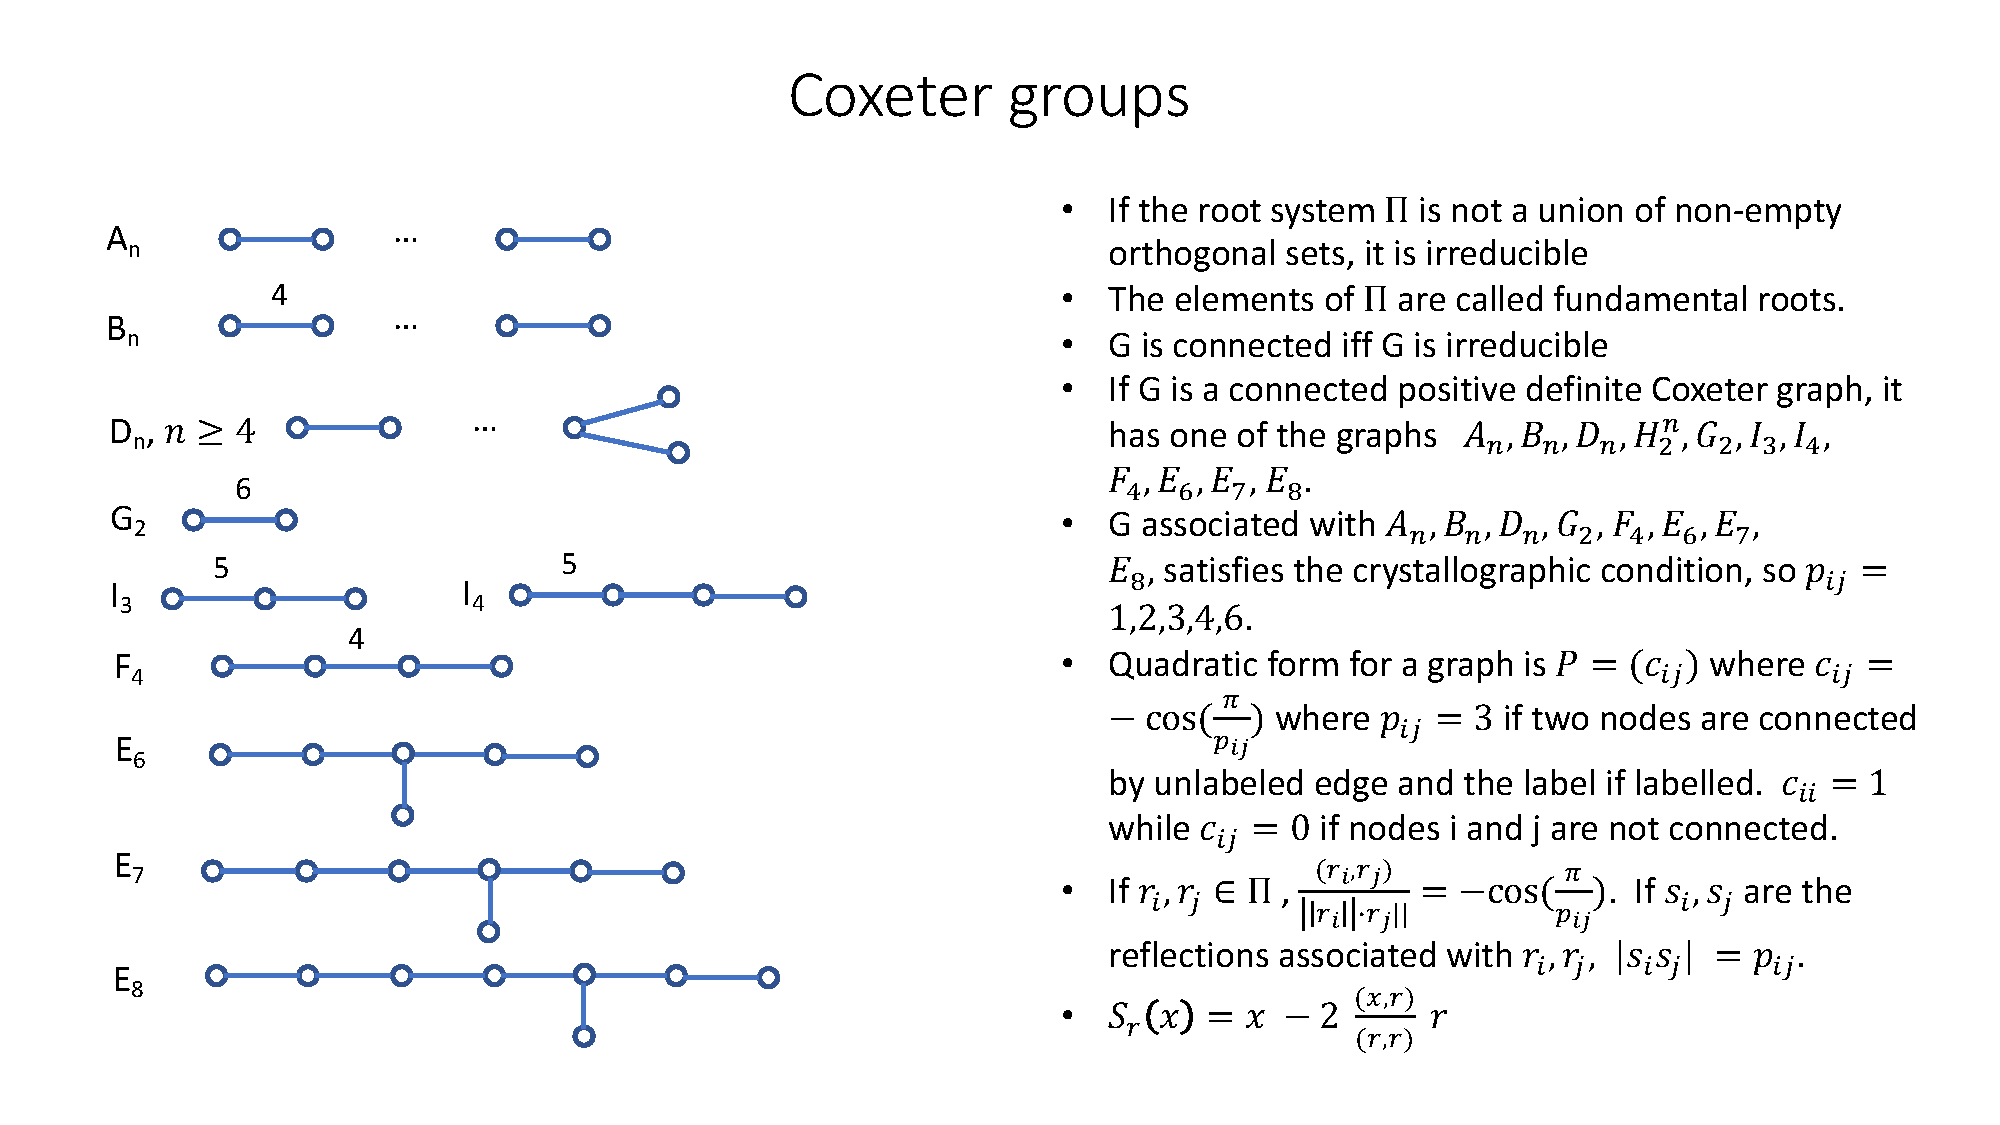
\includegraphics[natwidth=642, natheight=610, width=80mm]{dynkin.pdf}
\end{figure}
{\bf Theorem 72:}
If $G$ is a connected positive definite Coxeter graph then $G$ is one of
$A_n$,
$B_n$,
$D_n$,
$H_2^n$,
$G_2$,
$I_3$,
$I_4$,
$F_4$,
$E_6$,
$E_7$, or
$E_8$.
\begin{quote}
\emph{Proof:}  
The graph for $G$ can contain no cycles or the form would not be positive definite.
If $H_2^n$ is a subgraph of $G$, for any $n \ge 7$ then $G= H_2^n$ otherwise
$U_3$  would be in the graph.  Similarly, $G= G_2$ if it occurs.
We can assume any branch is labeled $3$, $4$ or $5$.  Suppose that $B_2$
is a subgraph of $G$; it cannot occur more than twice otherwise some $S_n$
would be a subgraph.  $G$ cannot have a branch point otherwise $T_n$ would be
a subgraph.  If $H_2^5$ is a subgraph then $G= H_2^5$, $G= I_3$ or
$G= I_4$.  There are no other possibilities otherwise $G$ would have $Z_4$
or $Y_5$ as a subgraph.  If $B_2$ is a subgraph but $H_2^5$ is not, then
$G$ may be $B_n$ for some $n \ge 2$ or $F_4$.  There are no other possibilities
otherwise $V_5$ would be a subgraph of $G$.  In the case that all branches are unmarked
then $G$ can have at most one bransh point and only $3$ branches can emanate from any branch point
otherwise $Q_n$ would occur in $G$.  If there is no branch point $G= A_n$.  If $G$
has one branch point, $G= D_n$ for some $n$ or $G= E_6, E_7, E_8$ or $R_7, R_8, R_9$ would
occur in $G$.
\end{quote}
{\bf Theorem 73:}
If $G$ has Coxeter graph
$A_n$, $B_n$, $D_n$, $H_2^n$,
$G_2$, $I_3$, $I_4$, $F_4$,
$E_6$, $E_7$, or
$E_8$ then $G$ satisfies the crytallographic condition.
\begin{quote}
\emph{Proof:}  
${\cal L} = \sum_{i-1}^n k_i r_i$.  If $p_{ij}= 3$, $||r_i||= ||r_j||$ and
$(r_i , r_j ) = - {\frac 1 2} ||r_i|| \cdot ||r_j||$ and $s_i(r_j)= r_i + r_j \in {\cal L}$.
If $p_{ij}= 4$, $s_i(r_j)= r_j + r_i$ or $s_i(r_j)= r_j + 2r_i$.
If $p_{ij}= 6$, $s_i(r_j)= r_j + r_i$ or $s_i(r_j)= r_j + 3r_i$.
If $p_{ij}= 1$, $s_i(r_j)= - r_j$.
If $p_{ij}= 2$, $s_i(r_j)= r_j$.
\end{quote}
\begin{center}
\begin{tabular} {|r|r|}
\hline
{\bf Graph} & {\bf Base} \\
\hline
$A_n$ & $r_i= e_{i+1}-e_i$, $1 \le i \le n$ \\
\hline
$B_n$ & $r_1= e_1$, $r_i= e_{i}-e_{i-1}$, $2 \le i \le n$ \\
\hline
$D_n$ & $r_1= e_1 + e_2$, $r_i= e_{i+1}-e_i$, $2 \le i \le n$ \\
\hline
$H_2^n$ & $r_i= e_{i+1}-e_i$, $2 \le i \le n$ \\
\hline
$G_2$ & $r_i= e_2-e_1$, $r_2 = e_1 -2e_2+e_3$ \\
\hline
$I_3$ & 
$r_1= \beta(2 \alpha + 1, 1, -2 \alpha)$,
$r_2= \beta(-2 \alpha - 1, 1, 2 \alpha)$,
$r_3= \beta(2 \alpha, -2 \alpha -1 , 1)$\\
\hline
$I_4$ & $r_1= \beta(2 \alpha + 1, 1, -2 \alpha, 0)$, $r_2= \beta(-2 \alpha - 1, 1, 2 \alpha, 0)$,\\
 & $r_3= \beta(2 \alpha, -2 \alpha -1 , 1, 0)$, $r_4= \beta(2 \alpha, 0, -2 \alpha -1 , 1)$ \\
\hline
$F_4$ & 
$r_1= 1{\frac 1 2} (\sum_{i=1}^4 e_i$, $r_2= e_1$, $r_3= e_2 - e_1$, $r_4= e_3- e_2$ \\
\hline
$E_6$ & $r_1= 1{\frac 1 2} (\sum_{i=1}^3 e_i - \sum_{i=4}^8 e_i)$, $r_i= e_i-e_{i-1}$, 
$2 \le i \le 6$ \\
\hline
$E_7$ & $r_1= 1{\frac 1 2} (\sum_{i=1}^3 e_i - \sum_{i=4}^8 e_i)$, $r_i= e_i-e_{i-1}$, 
$2 \le i \le 7$ \\
\hline
$E_8$ & $r_1= 1{\frac 1 2} (\sum_{i=1}^3 e_i - \sum_{i=4}^8 e_i)$, $r_i= e_i-e_{i-1}$, 
$2 \le i \le 8$ \\
\hline
\end{tabular}
\end{center}
\begin{center}
\begin{tabular} {|r|r|r|}
\hline
{\bf Base} & $|\Delta|$ & {\bf Root System} \\
\hline
$A_n$ & $n^2+n$ & $\pm (e_i - e_j)$ \\
\hline
$B_n$ & $2n^2$ &
$\pm e_i$, $\pm e_i \pm e_j$ \\
\hline
$D_n$ & $2n(n-1)$ &
$\pm e_i \pm e_j$ \\
\hline
$H_2^n$ & $2n$ &
$(cos({\frac {j \pi} {n}}), sin({\frac {j \pi} {n}})) $, $0 \le j <2n$\\
\hline
$G_2$ & $12$ & $\pm(e_i - e_j)$, $1 \le i \le 3$, $ \pm (1, -2, 1)$, $(-2, 1,1)$, $\pm(1,1, -2)$ \\
\hline
$I_3$ & $30$ &
$ \pm e_i$, $1 \le i \le 3$, $\beta ( \pm (2 \alpha +1), \pm 1, \pm 2 \alpha)$,\\
& &  and all even permutation of coordinates\\
\hline
$I_4$ &  $120$ & $ \pm e_i$, $1 \le i \le 4$, $\beta ( \pm 2 \alpha , 0,  \pm (2 \alpha +1) )$, \\
& &  and all even permutation of coordinates\\
\hline
$F_4$ &  $48$ &
$ \pm e_i$, $\pm e_i \pm e_j$, $1 \le i \le 4$ \\
\hline
$E_8$ & $240$ &
$ \pm e_i \pm e_j $, $1 \le j < i \le 8$, $\sum_{i=1}^8 \epsilon_i e_i$, $\epsilon_i = \pm 1$,
$\prod_{i=1}^8 \epsilon_i = -1$ \\
\hline
$E_7$ & $126$ & roots of $E_8$ orthogonal to $u= (1,1,1,1,1,1,1,-1)$ \\
\hline
$E_6$ & $72$ & roots of $E_8$ orthogonal to $r_8= e_8 - e_7$ \\
\hline
\end{tabular}
\end{center}
\begin{center}
\begin{tabular} {|r|r|}
\hline
{\bf Graph} & $|G|$ \\
\hline
$A_n$ &  $(n+1)!$ \\
\hline
$B_n$ &  $2^n n!$ \\
\hline
$D_n$ &  $2^{n-1} n!$ \\
\hline
$H_2^n$ & $2n$ \\
\hline
$G_2$ &  $12$ \\
\hline
$F_4$ &  $2^{7} \cdot 3^{2}$ \\
\hline
$I_3$ &  $2^{3} \cdot 3 \cdot 5$ \\
\hline
$I_4$ &  $2^{6} \cdot 3^{2} \cdot 5^2$ \\
\hline
$E_6$ &  $2^{7} \cdot 3^{4} \cdot 5$ \\
\hline
$E_7$ &  $2^{10} \cdot 3^{4} \cdot 5 \cdot 7$ \\
\hline
$E_8$ &  $2^{14} \cdot 3^{5} \cdot 5^2 \cdot 7$ \\
\hline
\end{tabular}
\end{center}
\section{Mathieu Groups}
{\bf Construction:}
$M_{11}$: $\pi_1= (123)(456)(789), \pi_2= (147)(258)(369)$,
$ \langle \pi_1, \pi_2 \rangle = {\mathbb Z}_3 \times {\mathbb Z}_3$, 
$\rho_1= (2437)(5698), \rho_2= (2539)(4876)$, $ \langle \rho_1 , \rho_2 \rangle = Q \cong Q_8$.  Set
$M_9= \langle \pi_1 , \pi_2 , \rho_1 , \rho_2 \rangle $, $|M_9|=72$.  
Now set $\sigma= (1, 10)(4,5)(6,8)(7,9)$, $\mu= (4,7)(5,8) (6,9) (10,11)$,
$\theta= (4,9) (5,7) (6,8)(11,12)$.  
$M_{10}= M_9 \cup M_9 \sigma M_9$,  $(M_{10})_x= M_{9}$,
$M_{11}= M_{10} \cup M_{10} \mu M_{10}$,  $(M_{11})_x= M_{10}$,
$M_{12}= M_{11} \cup M_{11} \theta M_{11}$,  $(M_{12})_x= M_{11}$.  $|M_{11}|=7920$.
\\
\\
{\bf Theorem 74:}
$|M_{24}|= 24 \cdot 23 \cdot 22 \cdot 21 \cdot 20 \cdot 48 $.  $M_{11}$ is simple.
\begin{quote}
\emph{Proof:}
Let $N$ be a non-trivial normal subgroup, it is regular and all Sylow 11 subgroups
are contained in it (there are 144 by Sylow) and $|G:N|= 5$.  All Sylow 3 subgroups
of $M_{11}$ are in $N$ and $\psi= \pi_1 \sigma \pi_2^2 \sigma^{-1}$ has order 5 which is a
contradiction.  Note that the symmetries of $S(4,5,11)$ also generate it and
that $(M_{11})_a= PSL_2(9)$ and $(M_{22})_a = PSL_3(4)$.
\end{quote}
\section{Conway's Groups}
{\bf Notation:}  Let $R(C)$ be the row space of $C$ over $GF(2)$.  Define the $\Gamma$ to
be the collection of $(v_1, v_2, \ldots , v_{24})=v \in {\mathbb Z}^{24}$ such that
(1) $\sum_{i=1}^{24} v_i = 4m$, (2) $v_i = m \jmod{4}$, 
if $c_i = 0$, (3) $v_i=m+2 \jmod{4}$ if $c_i = 1$.
\\
\\
{\bf Definition 18:}
$L_8 \rightarrow \Lambda_8$:  $v \in \Gamma_8$ iff
$v \in L_8$ and $\sum_{i=1}^{8} v_i = 4m$.  Contact number: $112+128=240$, radius: ${\sqrt 2}$.
\emph{Alternate definition} of $\Lambda_8$: $8$-tuples whose spheres are congruent $\jmod{2}$ to
rows of $A_8$ or ${\overline {A_8}}$.
Density is ${\frac {\pi^4}{4!2^4}}$.
\\
\\
{\bf Golay:}
$L_8$:  $v \in L_8$ iff $v \in {\mathbb Z}^8$ and $v_i = a_i \jmod{2}$ or
$v_i = {\overline a_i} \jmod{2}$.  Generator matrix:
$$\left(
\begin{array}{cccccccc}
1 & 1 & 1 & 1 & 1 & 1 & 1 & 1 \\
2 & 0 & 0 & 0 & 0 & 0 & 0 & 0 \\
0 & 2 & 0 & 0 & 0 & 0 & 0 & 0 \\
\ldots & \ldots & \ldots & \ldots & \ldots & \ldots & \ldots & \ldots \\
0 & 0 & 0 & 0 & 0 & 0 & 2 & 0 \\
\end{array}
\right).$$
{\bf Definition 19:}
Let $R(C)$ be the row space of ${\cal G}_{24}$ over $GF(2)$.  
Define the \emph{Leech Lattice}, $\Lambda_{24}$,
as the vectors that satisfy the following conditions:
Express coordinates in $E_{24}$ in binary and retain the ones that satisfy
the following conditions (a) the $24$ $1$'s bits are either all $0$ or all $1$, (b)
the $2$'s bits form a row in $R(C)$, (c) $4$'s bits rows have even parity for points
with $1$'s bits that are all $0$ and odd otherwise. This is equivalent to the following:
Suppose ${\vec c} \in R(C)$ and for $m \in {\mathbb Z}$, define
${\vec c}(m)= \{  
v \in {\mathbb Z}^{24}:  \sum_i v_i = 4m, 
c_i = 0 \rightarrow v_i = m \jmod{4},
c_i = 1 \rightarrow v_i = m+2 \jmod{4}
\}$,
$\Lambda = \Lambda_{24}= \cup_m {\vec c}(m)$.
\\
\\
{\bf Theorem 75:}   In $\Lambda$, lattice points are seperated by a minimum
distance of $4 {\sqrt 2}$.  Lattice points a minumum distance from the origin
have shapes: $(0^{16}, (\pm 2)^8)$, $(0^{22}, (\pm 4)^2)$, $((\pm 1)^{23}, (\pm 3))$.  
Hence the contact number is $98256$ (lattice point with even parity) + $98304$ 
(lattice point with odd parity) $= 196,560$;  
the density is $.001929$.  Each pair of adjacent lattice points is adjacent to $4600$
others. \emph{Example:} $(4,4, 0, \ldots, 0)$
is adjacent to $(4,0, \ldots , 0)$ - there are $88$ of these,
$(2,2, \ldots , 0)$ - there are $77 \times 2^7$ of these and
$(1,3, \ldots , 0)$ - there are $2048$ of these.
For the first Leech packing,
the density is ${\frac {2^{24}} { 2 \times 2^{12}}}= 2^{-11}$, 
first factor of $2$ in 
denominator is from condition that the sum of the
coordinates $= 0 \jmod{4}$ and so the packing density is $.0009647$.  The
Leech lattice doubles this which is about $.8$ of the Rogers bound.
\\
\\
Noting that there must be an even number of $-2$'s,
for the Leech packing, lattice points with even coordinates are:
\begin{center}
\begin{tabular} {|r|r|}
\hline
{\bf Shape} & {\bf Number} \\
\hline
$0^{16}, (-2)^8$ & $759$ \\
$0^{16}, (-2)^6, 2^2$ & $759 \cdot {8 \choose 2}=21252$ \\
$0^{16}, (-2)^4, 2^4$ & $759 \cdot {8 \choose 4}=53130$ \\
$0^{16}, (-2)^2, 2^6$ & $759 \cdot {8 \choose 2}=21252$ \\
$0^{16}, 2^8$ & $759$ \\
$0^{22}, (-2)^2$ & ${24 \choose 2}=276$ \\
$0^{22}, -2, 2$ & $ 24 \cdot 23 =552$ \\
$0^{22}, 2^2$ & ${24 \choose 2}=276$ \\
\hline
{\bf Total} & $98256$\\
\hline
\end{tabular}
\end{center}
The lattice points with odd coordinates are:
\begin{center}
\begin{tabular} {|r|r|}
\hline
{\bf Shape} & {\bf Number} \\
\hline
$(-1)^{23}, 3$ & $24$ \\
$(-1)^{16}, (1)^{7}, -3$ & $759 \cdot 8= 6,072$ \\
$(-1)^{15}, (1)^{8}, 3$ & $759 \cdot 16= 12,144$ \\
$(-1)^{12}, (1)^{11}, -3$ & $2576 \cdot 12= 30,912$ \\
$(-1)^{11}, (1)^{12}, 3$ & $2576 \cdot 12= 30,912$ \\
$(-1)^{8}, (1)^{15}, -3$ & $759 \cdot 16= 12,144$ \\
$(-1)^{7}, (1)^{16}, 3$ & $759 \cdot 8= 6,072$ \\
$(1)^{23}, -3$ & $24$ \\
\hline
{\bf Total} & $98304$\\
\hline
\end{tabular}
\end{center}
There are 
$4600$ vertices adjacent to $2$ adjacent simplex,
$891$ vertices adjacent to $3$ adjacent simplex,
$336$ vertices adjacent to $4$ adjacent simplex and
$170$ vertices adjacent to $5$ adjacent simplex.  
This gives a dihedral like estimate on the size of the symmetry group.
\\
\\
{\bf Definition of
Conway's group:} ${\bf .O}$ is the set of rotations in ${\mathbb R}^{24}$ fixing $O$ 
pointwise and $\Lambda$ setwise.
\\
\\
{\bf Notation:}
$v_S= \sum_{i \in S} v_i$. 
$Q= \{ x^2: x \in F_{23} \}, N= \Omega \setminus Q$.
$A+B= A \setminus B \cup B \setminus A$.  $N_i= \{ n-i, n \in N \}$.  Golay code,
${\cal C}$, is
generated by $N_i, N_{\Omega}$.  $N_A = \sum_{a \in A} N_a$.  $C \in {\cal C}$ iff $N_C=0$.
$\Omega= PL(23)$, $\alpha: x \mapsto x+1$, $\beta: x \mapsto 2x$,
$\gamma: x \mapsto {\frac {-1} x}$, 
$\delta: x \mapsto 9 x^3, x \notin Q$ and
$\delta: x \mapsto {\frac {x^3} 9}, x \in Q$.  
$L_2(23)= PSL_2(23)= \langle \alpha, \gamma \rangle$,
$M_{24}= \langle \alpha, \gamma, \delta \rangle$.  If $\pi \in S_{\Omega}$, define
$(v_i)^{\pi} = v_{\pi(i)}$.  
$\epsilon_S(v_i) = -v_i, i \in S$ and
$\epsilon_S(v_i) = v_i, i \notin S$.
\\
\\
{\bf Theorem 76:}
The set $G \Lambda = \{ 2 v_K, K \in R(C) \} \cup
\{ v_{\Omega} - 4 v_{\infty} \}$ generates $\Lambda$.  If $v, w \in G \Lambda$, then
$v \cdot v= 16n$ and $v \cdot w = 0 \jmod{8}$.  
$\Lambda_n= \{ x  \in \Lambda, x \cdot x = 16n \}$.  $\Lambda_1 = \emptyset$,
$\Lambda_2$ consists of 
$\Lambda_2^2$ of shape $(0^{16}, (\pm 2)^8)$ - there are $97152$ of these,
$\Lambda_2^3$ of shape $((\pm 1)^{23}, (\pm 3)^1)$ - there are $98,304$ of these,
$\Lambda_2^4$ of shape $(0^{22}, (\pm 4)^2)$ - there are $1104$ of these.
In tabular form:
\begin{center}
\begin{tabular} {|r|r|r|}
\hline
{\bf Name} & {\bf Shape} & {\bf Number} \\
\hline
$\Lambda_2^2$ & $0^{16}, \pm 2^8$ & $759 \cdot 2^7$\\
\hline
$\Lambda_2^3$ & $\pm 1^{22}, \pm 3$ & $24 \cdot 2^{12}$\\
\hline
$\Lambda_2^4$ & $0^{22}, \pm 4^4$ & ${24 \choose 2} \cdot 2^2$\\
\hline
\end{tabular}
\end{center}
{\bf Notation:}
If $S \in R(C)$, $\epsilon_S \in .O$.
$E= \langle \epsilon_S \rangle_{S \in R(C)}$, $M= M_{24}$.  $N= EM$.
$T_0= \{0, 3, 15, \infty \}$,
$T_1= \{ 1,12,21,22 \}$,
$T_2= \{ 2,7,11,13 \}$,
$T_3= \{ 4,10,16,17 \}$,
$T_4= \{ 5,6,9,19 \}$,
$T_5= \{ 8, 14,18,20 \}$,
$B= \{ T_0, T_1, T_2, T_3, T_4, T_5 \}$.
\\
\\
{\bf Theorem 77:}
$\lambda \in .O$ and $\lambda$ fixes $v_i$ (some $i$) iff $\lambda \in N$.
\begin{quote}
\emph{Proof of $\rightarrow$:}
Suppose $\lambda \in .O$ and $\lambda(v_i)= v_i$.  If $\lambda(v_j)= w_j, i \ne j$ then
$(v_i, w_j)= 0$.  Since $4 v_i + 4 v_j \in \Lambda_2$,
$4 v_i + 4 w_j \in \Lambda_2$.  Examining the elements of $\Lambda_2$, we see
$w_j= \pm v_k$ for some $k \in \Omega$ since $8w_j \in \Lambda$ and $4w_j \notin \Lambda$.
Distinct values of $j$ yield distinct values of $k$.  Thus $\lambda= \pi \epsilon_S$,
$S \subseteq \Omega, \pi \in S_{24}$.  The non-zero coordinates of
$\lambda( 2 v_K ), K $ an octet are in the coordinate postions $\pi(K)$, so
$\pi(K)$ is an octet and  $\pi \in M_{24}=M$.  $\lambda( v_{\Omega} - 4 v_{\infty})$ is
a lattice point of the same shape and the coordinates are $=1 \jmod{4}$.
$\epsilon_S: v_i \mapsto -v_i, i \in S$ so the coordinates of
$\lambda( v_{\Omega} - 4 v_{\infty})$ which are $= 3 \jmod{4}$ are in the places
$\pi(S)$ and so $S \in R(C)$.  So $\lambda = \pi \epsilon_S \in N$.
\end{quote}
{\bf Theorem 78:}
If $\lambda(\Lambda_2^4)= \Lambda_2^4$ then
$\lambda \in N$.
\begin{quote}
\emph{Proof:}
We use the following lemma:
\\
\emph{Lemma:} If $\lambda \in .O$ and $|\lambda|= p$, a prime then $p \le 23$ further,
no element of $.O$ has order $13 \cdot 23$.
\\
\\
Let $H$ be the symmetries fixing $\Lambda_2^4$ as a whole and $x= 4v_i +4v_j$
and $N_x$ is the subgroup fixing $x$.  $N$ only changes signs and permutes
coordinates so $N: \Lambda_2^4 \rightarrow \Lambda_2^4$ and fixes
$\Lambda_2^4(x)$ as a whole.  There are $2^2 {22 \choose 2}= 924$ vectors
of the form $\pm 4 v_h \pm 4 v_k$ are perpendicular to 
$\pm(4 v_i - 4 v_j)$ with
$h, i, j,k$ distinct and so are
$\pm(4 v_i - 4 v_j)$.  These $926$ vectors form
$\Lambda_2^4(x)$.  $N_x$ is $2$-transitive so $\exists \sigma: 
(4 v_i - 4 v_j) \mapsto \pm (4 v_i - 4 v_j) $ and no other elements are in this orbit.
Thus $\{ (4 v_i - 4 v_j), -(4 v_i - 4 v_j) \} $ form a single orbit.
$N_x \subseteq H_x$ and the orbits of $H_x$ are a union of $N_x$ orbits.  As a result,
it is either all $926$ orbits or the $N_x$ orbits.  In the latter case,
$|H_x: H_{x,y}| = 926= 2 \cdot 463$ which contradicts the lemma.
So we know $H_x$ has $2$ orbits on $\Lambda_2^4(x)$ and maps 
$(4 v_i - 4 v_j)$ to itself or it's negative.  In the first case, $\lambda(v_i)= v_i$ and
$\lambda \in N$ by the
previous theorem.  In the second case, $\lambda( v_i)= v_j$ and hence
$ (4 v_i + 4 v_h)  \mapsto (\pm 4 v_j \pm 4 v_k) , h \ne j $ and again $\lambda \in N$.  Thus
$H_x \subseteq N$ and $H_x \subseteq N_x$ and therefore $H \subseteq N$.
\end{quote}
{\bf Theorem 79:}
There is a subgroup isomorphic to $L_2(23)$ which is
transitive on octads. 
\begin{quote}
\emph{Proof:} 
There is a copy of $L_2(23)$ in $M_{24}$.
\end{quote}
{\bf Definition 20:} $\epsilon(v_i) = 
v_i \textnormal{ if } i \notin Q \textnormal{ and } -v_i \textnormal{ if } i \in Q $.
\\
\\
{\bf Theorem 80:} $N= \langle \alpha, \beta, \gamma, \delta, \epsilon \rangle$.
\begin{quote}
\emph{Proof:} 
Applying permutations from the right, note $\epsilon_K= 
\epsilon \alpha  \delta \alpha  \epsilon \alpha^{-1} \delta^{-1} \alpha^{-1}$, 
$K= \{ 0,1,4,5,11,12,14,22 \}$.  If $L$ is another $8$-set and $\theta: K \rightarrow L$ then
$\epsilon_L = \theta^{-1} \epsilon_K \theta$.
\end{quote}
{\bf Theorem 81:}
$N$ is a proper subgroup of $.O$.
\begin{quote}
\emph{Proof:} 
Let $T=T_0$ be any $4$-set of $\Omega$.  $T$ lies in $5$, $8$ sets
$ T+T_1, T+T_2, \ldots, T+T_5$, where $T_i$ is the complement of
$T$ in the $i$-th $8$-set.  $\Omega$ is the disjoint union of
$6$, $4$-sets.  $B= \{ T_0 , T_1 , \ldots , T_5 \}$.
$\eta= \eta_B: v_i \mapsto v_i- {\frac 1 2} v_{T_j}$ and
$\zeta_T= \eta \epsilon_T$.  $\zeta_T^2=1$.  $\zeta_T \in .O$ and
$\zeta_T \notin N$.
\end{quote}
{\bf Theorem 82:}
$H_x$ is transitive on $\Lambda_2(x)$.
\begin{quote}
\emph{Proof:} 
Let $x= v_{\Omega}- v_{\infty}$.  The order of each orbit of $H_x$ on $\Lambda_2(x)$
has order divisible by $23$.
\end{quote}
{\bf Theorem 83:}
If $H>N$, $H$ is transitive on $\Lambda_2$ and $H=.O$.  $|.O|=
2^{22} \cdot 3^{9} \cdot 5^4 \cdot 7^2 \cdot 11 \cdot 13 \cdot 23= 8,315,553,613,086,720,000$.
\begin{quote}
\emph{Proof:} 
(1) $\Lambda_2^2$, $\Lambda_2^3$, $\Lambda_2^4$ are all $N$-orbits.  
A counting argument shows that the union of two
of them can't be an $H$ orbit (otherwise, $p \mid |.O|$ for $p>23$).  Now define
$\Lambda_2 (x)= \{ y: y \in \Lambda_2, y \perp x \}$.
Recall $H_x$ is transitive on $\Lambda_2(x)$.
Since $M_{24}$ is $5-$transitive $|H_x : H_{x,y}|= 926$ and
$|.O|= |H| = 196560 \cdot |H_x|$; further,  $H_x$ is transitive on 
$\Lambda_2 (x)= \{ y: y \perp x \}$.  An orbit of $H_x$ has $93150$ elements so
$|H_x|= (93150) |H_{x,y}|$ and $H_{x,y} = E_{10} M_{22}$.  This gives the order of
$H$ and shows $H=.O$.
\end{quote}
{\bf Definition 21:}
For $x \in \Lambda_2$, define $\{ x , -x \}$ is called a diameter.
${\overline {\Lambda_2}}$ is the set of $98280$ diameters.
$.1= .O_d, d= \{x, -x \}, x \in \Lambda_2$ 
\\
\\
{\bf Theorem 84:} $N$ is maximal in $.O$.  $.O= \langle N, \zeta \rangle$.
\begin{quote}
\emph{Proof:} 
By the theorem, if $H>N$, $H=.O$.  The second statement follows from $\zeta \notin N$ and $\zeta \in .O$.
\end{quote}
{\bf Theorem 85:} 
$.O$ is transitive on ordered pairs of points of vectors of $\Lambda_2$ with a
given scalar product.
\begin{quote}
\emph{Proof:} 
$\Lambda_2= \{ v \in \Lambda: v \cdot v= 16 \cdot 2 \}$.  By looking at products of
vectors of standard type, the possible products are
$0, \pm 8, \pm 16, \pm 32$.  Put $\Lambda_2(x,m)= \{y: (x,y)= m \}$.
We find orbits of $N_x$ on $\Lambda_2(x,16)$ and show 
$\Lambda_2(x,16)$ is a single orbit of $.O_x$.
\end{quote}
{\bf Observation:}
Let $\varphi$ be an octad, say $\{ 0,1,2,3,4,7,10,12 \}$,
and $i \notin \varphi$; suppose $K$ is the subgroup fixing $\varphi$,
setwise and $H= K_i$.  The subset fixed is of codimension $8$ so it has dimension $4$.  $K$
acts naturally on this $4$-dimensional subspace.  $K \approx 2^4 L_4(2)$.
\\
\\
{\bf Theorem 86:} 
$.1 \cong .O/{\mathbb Z}(.O)$ and
$|{\mathbb Z}(.O)|= 2$.
\begin{quote}
\emph{Proof:} 
Suppose $\lambda \notin \{\pm1\} \in {\mathbb Z}(.O)$.
$\theta_i= \alpha^{23-i} \gamma \alpha  \gamma \alpha^i $ fixes $i$ and moves all other
points of $\Omega$.  
(1) $\lambda$ cannot send $v_j \mapsto \pm v_j, \forall j$ since
$(v_j)\lambda \alpha = - v_{j+1}$ and
$(v_j)\alpha \lambda= v_{j+1}$.  
(2) $\lambda$ cannot map $v_i \mapsto \pm v_j, i \ne j$, 
$(v_i) \lambda \theta_i= \pm (v_j) \theta_i= \pm v_k \ne \pm  v_j$, but
$(v_i) \theta_i \lambda= \pm (v_j)$.
(3) Remaining case, namely, $\lambda: v_i \mapsto w \ne \pm v_j, j \in \Omega$ is impossible too.
If $(v_j)\lambda = w \ne \pm v_k$, any $k$.  $(8v_i)\lambda \in \Lambda_4$ and has one of the following
form $(0^{23},\pm 8^{1})$, $(\pm 0^{20},\pm 4^{4})$, $(\pm 0^{16},\pm 2^{7}, \pm 6^{1})$,
$(\pm 0^{14},\pm 2^{8}, \pm 4^{2})$, $(\pm 0^{11},\pm 2^{12}, \pm 4^{1})$, $(\pm 0^{8},\pm 2^{16})$,
$(\pm 1^{21},\pm 3^{2}, \pm 5^{1})$, $(\pm 1^{19},\pm 3^{5})$.  The only one fixed by $\theta_i$ is
$8v_i$.  Thus
$(v_i) \lambda \theta_i = (w)\theta_i \ne w$ but
$(v_i) \theta_i \lambda= w$ and the theorem holds.
\end{quote}
{\bf Theorem 87:}
$.1$ acts primitively on ${\overline {\Lambda_2}}$.
\begin{quote}
\emph{Proof:} 
Each element of $.1$ permutes $98280$ diameters.  Since $.O$ is transitive on
$\Lambda_2$, $.1$ is transitive for diameters.  Suppose
$.1$ is imprimitive.  $|S_1| \mid 98280$.  Let ${\overline x} \in S_1$.
Since $|S_1| \ge 1, \exists y \in S_1$ whose orbit under $.1_{\overline x}$
has order $4600, 47104, 46575$.  Since $.1$ fixes ${\overline x}$,
$.1: S_1 \rightarrow S_1$ and $|S_1| \ge 4601$.  None divide
$98280$ so $\exists {\overline z} \ne {\overline x}$ outside $S_1$.
But then $S_1$ which has at least $1+4600+46575=51176$ and thus must be all of
${\overline {\Lambda_2}}$.  This contradicts the assumed imprimitivity of $.1$.
\end{quote}
{\bf Theorem 88:}
$.1= .O/{\mathbb Z}(.O)$ is simple.
\begin{quote}
\emph{Proof:} 
Suppose ${\mathbb Z}(H) \subsetneq H \subsetneq .O$.  
(1) $H$ is transitive on ${\overline {\Lambda_2}}$.
If not $\exists {\overline x}= \{x, -x\}$
and $y \in \Lambda_2: \eta(x)= y, \eta \in H$.  $.O$ is transitive on
${\overline {\Lambda}}_2$.  Orbits of $H$ in ${\overline {\Lambda}}_2$ are of
equal size.
(2) $N$ is not normal in $.0$.  This is proved by looking at $B$, the $4$-subsets defined above.
(3) $H=N$.  $|H:H_x|= 13 \cdot 7560$.  Let $P \in S_{13}$.  Since $H$ is normal, all the sylow $13$
subgroups of $.O$ are in $H$ so
$|>O:N_{.O}(P)= |ccl_{.O}(P)|=
|ccl_{H}(P)|= |H:N_H(P)|$ and $|.O:H|= |N_{.O}(P):N_H(P)|$ with $N_H(P)= N_{,O}(P) \cap H$.
Thus $|.O|= |N_{.O}(P)H|= {\frac
{|N_{.O}(P)| \cdot |H|}
{|N_{.O}(P) \cap H|}}$ and
$23 \mid |N_{.O}(P)|$ or $23 \mid |H|$.  In the former case, put
$K= \langle \lambda \rangle$,
$P= \langle \mu \rangle$, $|\lambda|= 13$, but then $|PK|=13 \cdot 23$ which contradicts an
earlier lemma.  In the latter case,  $23 \mid |H|$ so $H \cap N = N$ but $N$ is maximal so
$H=N$.
Now we have $H \lhd .O$ and $H=N$ but $N$ is not normal and this establishes the result.
$\zeta \in .1: x \mapsto z$,
$\lambda \in H: x \mapsto w$.
$\zeta(w)= \zeta(\lambda(x))= \zeta \lambda \zeta^{-1}(z)$ is in orbit of $z$
sinze $\zeta \lambda \zeta^{-1} \in H$.  $.1$ preserves orbits in
$\Lambda_2$ and the orbits are sets of imprimitivity for $.1$ on
${\overline {\Lambda}}_2$ which contradicts the previous result.
For $x \in {\overline {\Lambda}}_2$, 
$|H:H_x|=|{\overline {\Lambda}}_2| = 98280= 13 \cdot 7560$.
Let $P \in S_{13}(H)$ all such are $H$ conjugate and
$|.O:N_{.O}(P)|= |H:N_H(P)|$.
\end{quote}
{\bf Conway's other simple groups:} 
$.2= \{ x \in .O$, $x$ stabilizes
$2$ points $v,w \in \Lambda_2: |v-w|= 4 {\sqrt 2} \}$.
$.3= \{ x \in .O$, where $x$ stabilizes
$2$ points $v,w \in \Lambda_2: |v-w|= 4 {\sqrt 3} \}$.
